\chapter{Кого называли змеями?}

Слово «змий» в старину имело много значений.

Одно из них – бес, черт.

А как называли языческих богов после принятия на Руси христианства? Бесами, чертями. 

Умолчание имен языческих богов, да и вообще дохристианских представлений бытовало не токмо устно, но и в литературных памятниках. Летописцы то и дело обрывают себя на слове, поясняя: «не льзе казати срама ради».

Дело усложняется еще и многослойностью верований Славян, у которых, прежде подчинения их варягам-Руси, был культ покойников, предков. Поклонялись ли Перуну и Волосу в землях, отличных от исконной родины Рюрика, до пришествия туда соотечественников оного, неведомо. После пришествия – судя по народному календарю – да.

У греков сохранилась древняя литература – все эти мифы о богах и героях. Зевс, Гера, Геракл и прочие знакомы нам не по фольклорным записям, а по литературным произведениям, и бог весть, сколько там чего от народных представлений. Храмы, где поклонялись Зевсу, много веков лежат в развалинах! Греки давно христиане. Греческие пастухи не рассказывают былички про Зевса. Но, глядя на давние статуи, мы соотносим их с мифами и понимаем – это Афродита, это Гермес. Вот как их представляли себе греки того времени.

А как Славяне воображали себе Перуна в то время, когда ему поклонялась а хоть бы дружина Вещего Олега?

%В былинах и преданиях, когда говорится о змеях, речь идет вовсе не об драконах-ящерах, ужах, полозах и прочих рептилиях. Их на Руси обозначали ёмким словом «гады». Сказители, не называя точно поганских богов по именам, заменяют их на общее «змей», «змий», подразумевая – «бес». 


%Былинные богатыри – ребята сами по себе не всегда положительные, противопоставляются обычно "злу" – змеям. Нет героя-змея, он всегда посрамляется богатырем

%Наукой считается, будто нет мифов о «славянских богах» – Перуне и других. У прочих народов есть. Греческие боги Олимпа и мирские их отношения со смертными, египетский пантеон и так далее. Правда, подробные истории про Зевса и его родственников нам известны из давних, но всё же литературных источников, а не из фольклорных, но это разговор особый.


%Былины, сказания, где упомянуты змеи, и есть часть того цикла мифов, где, как и в греческих, боги и люди соседствуют в одном сюжете. Просто вместо, скажем, «бог Перун» говорится – Змей. И в подготовленном художниками воображении современного читателя возникает образ эдакого динозавра.

Нынче идола Перуна обычно представляют как украшенный резьбой деревянный столб с лицом. 

Открываем Радзивилловский список. Его датируют 15 веком, но полагают, что иллюстрации сделаны с подлинника а хоть бы и 11 века. Значит, есть вероятность, что мы увидим, как художник 11 века полагал себе персонажей, обстановку и – кумиров, то бишь статуи богов. Учтем конечно, что 11 век уже христианство, и божницы могли не сохраниться, но это всё же ближе к событиям, нежели наше время.

«Мужи Олега» приносят клятву Перуну, заключая договор с греками:

\begin{quotation}
Цесарь же Леон с Александром мир створиста с Ольгом, имешеся по дань, и роте заходивше межи собою, целовавше сами крест, а Ольга водиша и мужий его на роту по рускому закону: кляшася оружьем своим, и Перуном, богом своим, и Волосом, скотьим богом, и утвердиша мир.
\end{quotation}


\begin{center}
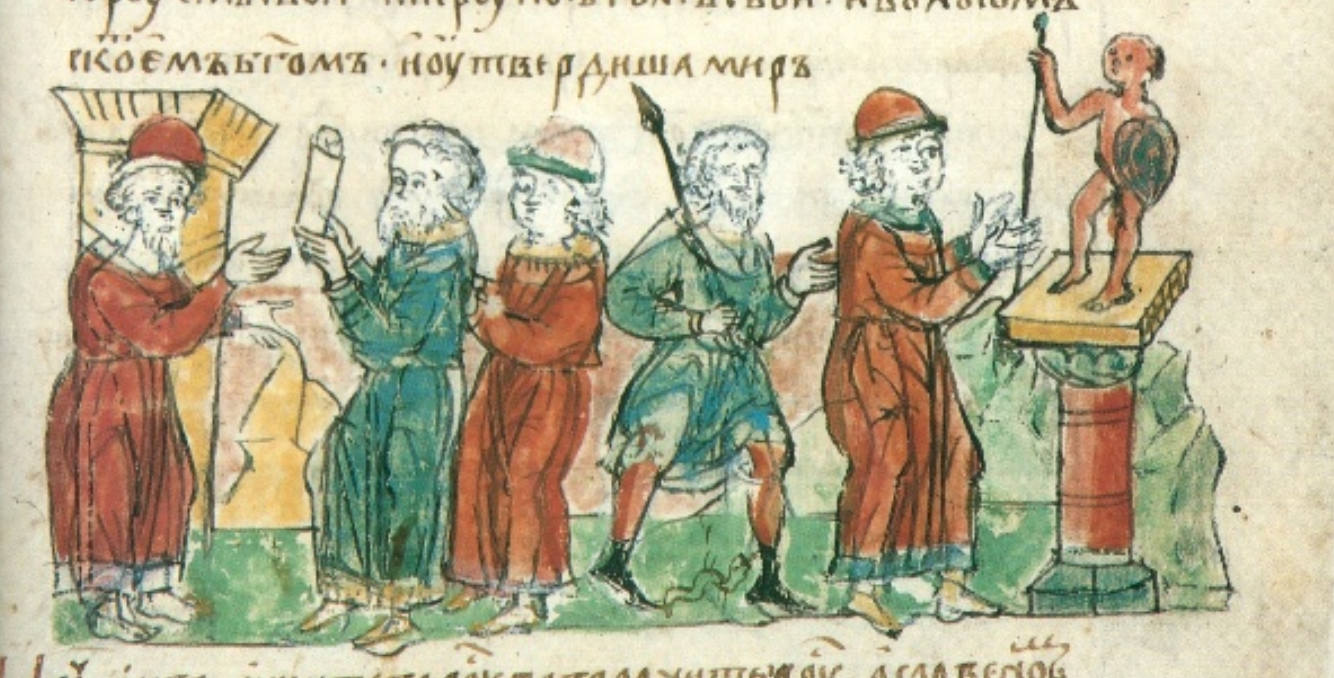
\includegraphics[width=\linewidth]{chast-zmiy/ktotakiezmei/rad-perun-01.jpg}
\end{center}

Вот как древний художник, хотя и не очевидец описываемых событий, изобразил кумира Перуна. Это, на постаменте-колонне, статуя человекоподобного существа. В одной его руке щит, в другой копье или посох. О размере статуи судить невозможно. Художники того времени любили уменьшать предметы, дабы они помещались на рисунке целиком. Мы видим либо такое уменьшенное стилистически изображение, или же статуя в самом деле была небольшого роста.

Крайний человек справа, рядом с Перуном – Вещий Олег, он же Ольг, Ольга (таким показан он и на предшествующей миниатюре, где берет дань, восседая на троне с подставкой для ног). Почему на постаменте стоит именно Перун, а не Волос? Следующая миниатюра подтвердит сопоставление, а покамест обратите еще внимание на змею под ногами второго справа человека.

Может это просто часть сцены, не имеющая значения. А возможно, намек художника на то, что человек – язычник. Однако, на других миниатюрах, при изображении поган, змеи уже не ползают, кроме изображения, на котором Олега кусает змея из конского черепа.

Следующая картинка показывает, что Игорь идет с послами на холмы, где стоит Перун:


\begin{center}
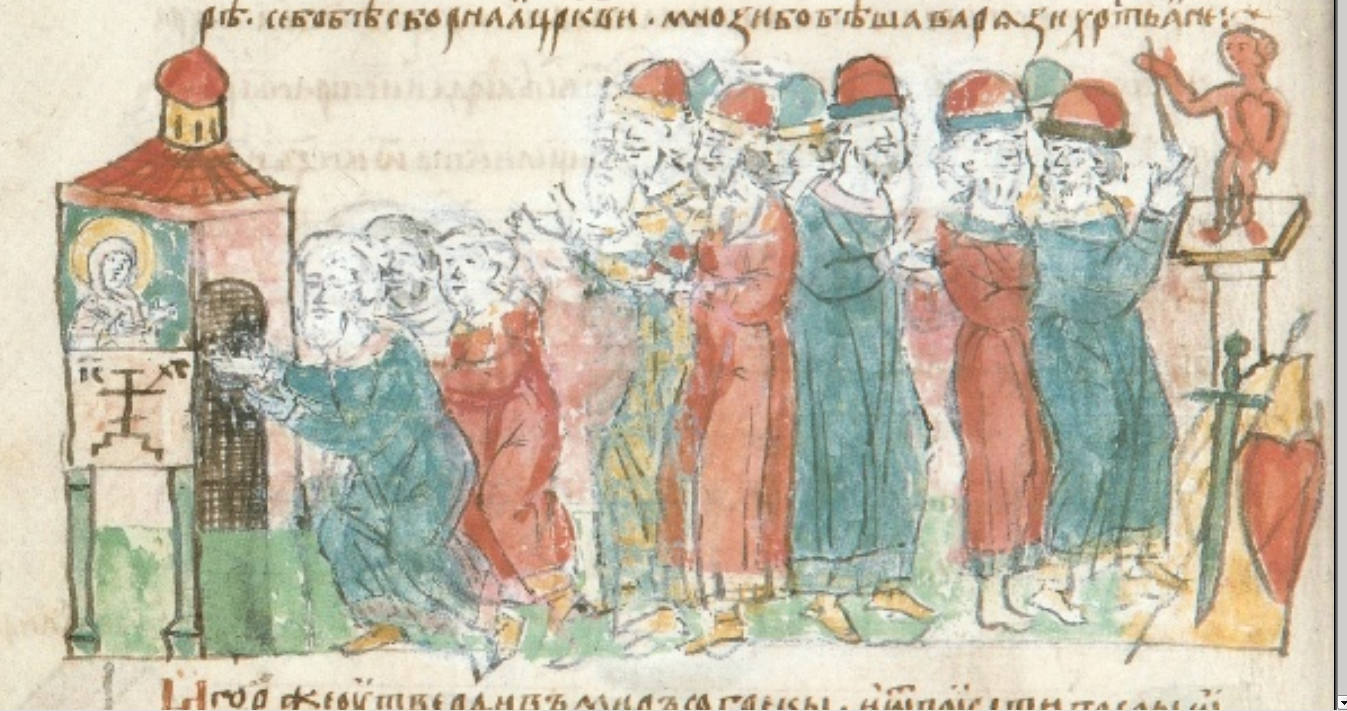
\includegraphics[width=\linewidth]{chast-zmiy/ktotakiezmei/rad-perun-02.jpg}
\end{center}

\begin{quotation}
И наутрея призва Игорь сли, и приде на холъмы, кде стояше Перун, и покладоша оружья своя, и щиты и золото, и ходи Игорь роте и мужи его, и елико поганыя руси, а хрестьяную русь водиша в церковь святаго Ильи, яже есть над Ручьем, конець Пасыньце беседы, и козаре: се бо бе сборная церкви, мнози бо беша варязи хрестьяни.
\end{quotation}


Игорь и его люди «ходи роте» – приносит клятву перед богами. С поганской частью Руси (дружины из числа народа варягов Руси) Игорь клянется перед Перуном, а с христианской частью этой Руси – в церкви Ильи. 

Наконец, третья картинка иллюстрирует летописный рассказ о том, как Владимир поставил кумиров на холме: «постави кумиры на холму вне двора теремнаго: Перуна древяна, а главу его сребрену, а ус злат, и Хрса, Дажьбога, и Стрибога, Симаргла, и Мокошь».

\begin{center}
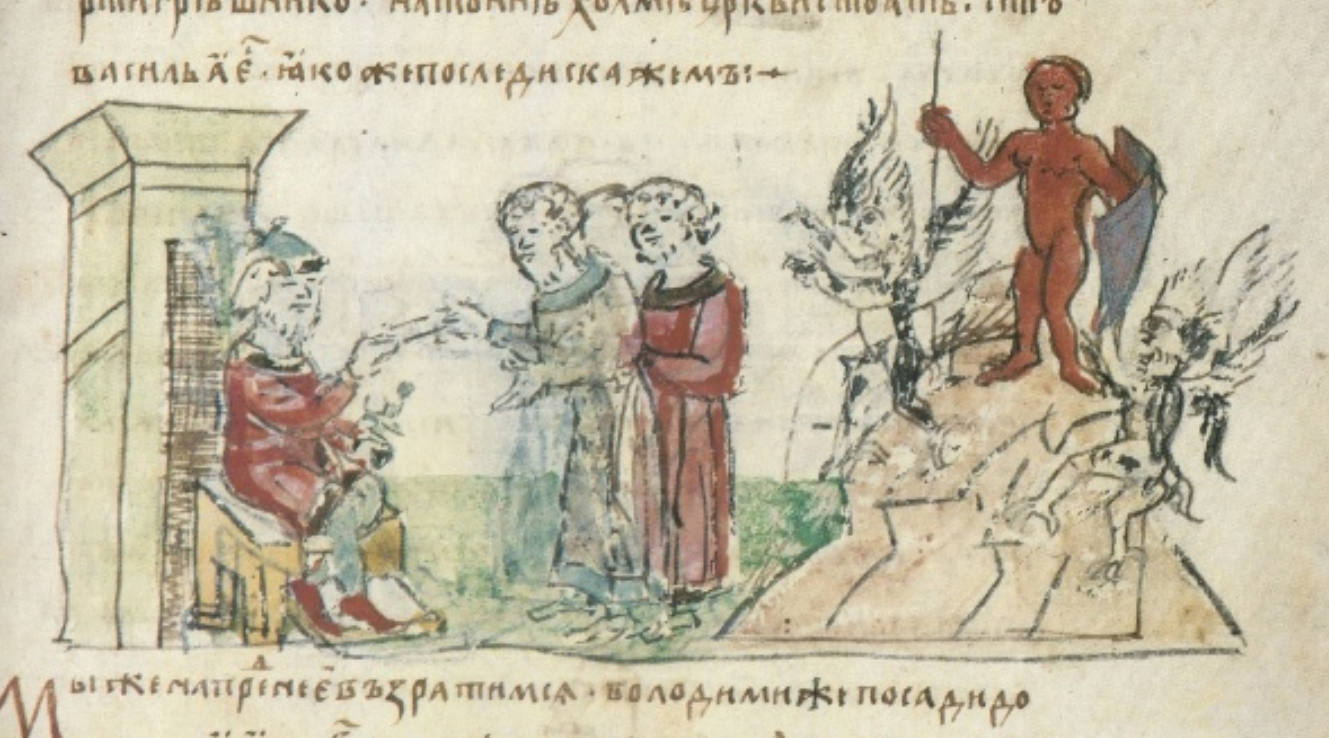
\includegraphics[width=\linewidth]{chast-zmiy/ktotakiezmei/rad-perun-03.jpg}
\end{center}

Здесь, как и ранее, идол Перуна не соответствует описанию из летописи. Он стоит на холме среди других кумиров. Отметим их крылья. Далее в той же Радзивилловской летописи, когда по сюжету уже принято христианство, сходным образом изображенные крылатые существа называются «бесами».

Начиная с двадцатого века, наукой упорно навязывалось мнение, что те идолы-колоды, которых находили археологи, и есть идолы Перуна. Будто на них это написано. В летописи описание кумиров другое? Ученых не волнует. На миниатюрах изображено другое? Ученых не волнует. Уже всё решили! А кумира из Радзивилловской летописи они называют «голым мальчиком» – при том, что пол, вообще говоря, по картинкам этим непонятен. А ведь художник не стеснялся в других случаях. Но идол Перуна нарисован без половых признаков, хотя, кажется, грудь его имеет скорее мужской вид. Вопрос, почему художник изображал кумира именно так, остается открытым.

Есть ли прямые подтверждения связи, что поганских богов именовали «змеями» в значении «бесы», а слово «змей» ставилось рядом с Перуном? Конечно.

В 1859 году Павел Якушкин записал\cite[стр. 118]{yakushin01} около новгородского Перынского скита историю о змияке-Перуне:

\begin{quotation}
 – Какой это столб стоит?  – спросил я старика, указывая на столб, очень похожий на верстовый, хотя большой дороги и не было. Мы в это время были под самым скитом Юрьевским, известным в народе под именем Перюньского. (это не совсем Перюньский и не совсем Перунский, а звук какой-то средний между у, ю и ы. В книгах монастырь называется Перынь)

 – А вот видишь ты, какое дело было,  – начал рассказчик,  – был зверь-змияка, этот зверь-змияка жил на этом самом месте, вот где теперь скит святой стоит, Перюньской. Кажинную ночь этот зверь-змияка ходил спать в Ильмень озеро с Волховскою коровницею. Перешел змияка жить в самый Новгород; а на ту пору и народился Володимер –  князь в Киеве; тот самый Володимер князь, что привел Руссею в веру крещеную. Сказал Володимер князь: «Всей земле русской – креститься». Ну и Новгороду тожь. Новгород окрестился. Чорту с Богом не жить: Новый Город схватил змияку-Перюна да и бросил в Волхов. Чорт силен: поплыл не вниз по реке, а в гору – к Ильмень-озеру; подплыл к старому своему жилью – да и на берег! Володимер князь велел на том месте церковь рубить, а дьявола опять в воду. Срубили церковь: Перюну и ходу нет! От того эта церковь назвалась Перюньскою; да и скит тоже Перюньской.

 – А столб-то какой?

 – Да на то и поставлен: место где, значит, Перюнь из Волхова выскочил. В Нове-городе, я помню, ставили столобочек, ставили с царем, так там солдаты в барабаны били, в музыку играли, честь отдавали, попы молебен пели. А здесь принесли солдатики столбушек, вкопали, да ушли. Да только не сказали народушку: какой такой с чего зародился той столобик. А ехали-то из Грузина: от Новагорода до Грузина считается 90 верст, 90 верст ехали со столобом и поставили столоб.

После я узнал, что этот «столобочек-памят\-ник» ни что иное как верстовой столб, поставленный водяною коммуникациею.
\end{quotation}

Про Перынь много чего уже написано, тьма домыслов, спорить с которыми не хочу. Но дабы не упрекнули в подтасовке изложения материала в пользу одного только, приведу историю из «Сказания о Словене и Русе», приложенном к Холмогорской летописи (Полное собрание русских летописей, том 33, Москва, 1977):

\begin{quotation}
Больший же сын оного князя Словена Волхв бесоугодник и чародей и лют в людех тогда бысть, и бесовскими ухищреньми мечты творя многи и преобразуяся во образ лютаго зверя коркодила, и залегаше в той реце Волхове путь водный, и непоклоняющих же ся ему овых пожираше, овых же изверзая и утопляя. 

Сего же ради людие, тогда невегласи, сущим богом окаяннаго того нарицая и Грома его, или Перуна, рекоша, руским бо языком гром перун именуется. 

Постави же он, окаянный чародей, нощных ради мечтаний и собирания бесовскаго градок мал на месте некоем, зовомо Перыня, иде же и кумир Перунов стояше. 

И баснословят о сем волхве невегласи, глаголющее, в боги сел\footnote{«сего»? – непонятно.} окаяннаго претворяюще. Наше же християнское истинное слово с неложным испытанием многоиспытане извести о сем окаяннем чародеи и волхове, яко зле разбиен бысть и удавлен от бесов в реце Волхове и мечтаньми бесовскими окаянное тело несено бысть вверх по оной реце Волхову и извержено на брег противу волховнаго его градка, иде же ныне зовется Перыня. 

И со многим плачем тут от неверных погребен бысть окаянный с великою тризною поганскою, и могилу ссыпаша над ним велми высоку, яко же обычай есть поганым. 

И по трех убо днех окаяннаго того тризнища проседеся земля и пожре мерзкое тело коркодилово и могила его просыпася с ним купно во дно адово, иже и доныне, яко ж поведают, знак ямы тоя не наполнися.
\end{quotation}
 
Толковать «Слово о Словене и Русе» трудно, как источник поздний и сборный, вероятно сильно правленный для ладности изложения. Старший сын Словена – Волхв – был бесоугодник и чародей. Он «бесовскими ухищреньми мечты творя многи». Слово «мечты» употреблялось встарь в значении призраков, видений наяву, чудес.

Также Волхв преобразовывался в «коркодила», залегал в реке и кто ему не поклонялся, того чародей пожирал или топил. Возможно, у Волхва было нечто вроде скафандра. Сказитель не знал, как его описать, и употребил «коркодил», как наиболее близкое известное ему по виду. Или речь шла в самом деле о каком-то ящере.

Народ подивился этим чудесам и поэтому решил, что Волхв – бог Перун, что значит «Гром». Сказитель, поздний по отношению к описываемому, вынужден пояснять, переводить сие слово. В месте Перыне, где стоял идол Перуна, Волхв построил себе «градок мал». Вероятно, решил оправдать народную молву о себе. Но попутно нарушил покой священного места.

Бесы удавили Волхва в реке Волхове и «мечтаньми бесовскими» перенесли его тело по течению вверх, выбросив на берег против волховного городка в Перыни. Погане похоронили чародея в кургане, три дня справляли тризну. После трех дней земля просела и тело «коркодилово» провалилось «во дно адово», и поныне (во времена рассказчика) был виден след от той ямы.

Сию историю часто хотят привязать ко крещению Новгорода, но про крещение есть три совершенно другие истории, без участия Волхва. В Новгородской первой летописи младшего извода, в Софийском временнике, да в Иоакимовской летописи, известной по выдержкам у Татищева. Я долго думал, цитировать или нет. Поскольку в главе и так много на первый взгляд лишнего, но любопытного материала, то думаю вреда не будет – тем более, что проявляется «технологичность» свергаемого идола Перуна, который говорил вполне осмысленные предложения.

Из Новгородской первой летописи младшего извода:

\begin{quotation}  
В лето 6497. Крестися Володимир и вся земля Руская; и поставиша в Киеве митрополита, а Новуграду архиепископа, а по иным градом епископы и попы и диаконы; и бысть радость всюду. 

И прииде к Новуграду архиепископ Аким Корсунянин, и требища разруши, и Перуна посече, и повеле влещи его в Волхово; и поверзъше уже, влечаху его по калу, биюще жезлеем; и заповеда никому же нигде же не прияти. 

И иде пидьблянин рано на реку, хотя горънци вести в город; сице Перун приплы к берви, и отрину и шистом: «ты, рече, Перунище, досыти пил и ял, а ныне поплови прочь»; и плы со света окошьное.
\end{quotation}

Из Софийского временника:

\begin{quotation}  
В лето 6497. Крестився Владимер и взя у Фотия патриарха царягородского единаго митрополита Киеву Леона, Новугороду архиепископа Акыма Корсунанина, а по иным градом епископы и попы и диаконы, иже крестиша всю землю Рускую; и бысть радость всюду.

И прииде Новугороду архиепископ Аким, и требища разори, и Перуна посече, и повеле влещи в Волхов; и поверзавше уже, влечахуть и по калу, биюще жезлием и пихающе. 

И в то время въшел бяше в Перуна бес: «О горе! Ох мне! Достахся немилостивым сим рукам». И вринуша его в Волхов. 

Он же пловя сквозе великы мост, (верже и палицу свою и рече: «На сем мя поминают новогородскыя дети»). Ею же и ныне безумнии, убивающеся утеху творять бесом. И заповеди никому же нигде не переяти его. 

И иде пидьблянин рано на реку, хотя горнеци вести в град; оли Перун приплы к берви, и отрину и шистом: «ты, рече, Перушице, до сыти еси пил и ял, а нынеча поплови прочь»; и плы света окошьное.
\end{quotation}  

Из Третьей Новгородской летописи – а тут уточняется, что свергаемый кумир стоял на Перыни:

\begin{quotation}
В лето 6496. Крестися великий князь Владимир Святославович, и взя у Фотия патриарха перваго митрополита Киеву Леона, а Новуграду епископа Иоакима Корсунскаго, а по иным градем епископы и попы и диаконы, иже крестиша всю землю Росийскую и бысть радость повсюду.

И прииде епископ Иоаким, и требища разори и Перуна посече, что в Великом Новеграде стоял на Перыни, и повеле повлещи в Волхов; и повязавше ужи, влечаху и по калу, биюще жезлием и пхающе, и в то время бяше вшел бес в перуна и нача кричати: о горе мне! ох! достахся немилостивым судиям (вариант: рукам) сим – и вринуша его в Волхов. 

Он же пловяше сквозь великий мост, верже палицу свою на мост, ею же безумнии убивающеся (вариант: упиющиеся либо убиющиеся) утеху творят бесом. И заповеда никому же нигде не переняти его.

И иде Пидблянин\footnote{Питьба, Пидьба – река в Новгородской области, приток Волхова. Любопытно, что Питьба течет параллельно Волхову, но в обратном ему направлении. Впадает в Волхов в пределах современного Новгорода, и вероятно «пидблянин» это житель местности возле устья, в описываемое время бывшего вне города.} рано на реку, хотя горницы везти в город, и перун приплыл к берегу, к бервы, и отрину его шестом, и рече ему: перунище! досыти еси ел и пил, а ныне прочь плыви – и плы из света некощное (варианты: 1. и плы света окошное; 2. преисподнее окно), сиречь во тму кромешную. 
\end {quotation}

Еще подробности. Добрыня, посланный Владимиром, поехал крестить Новгород – на это указывает Сокращенный летописный свод 1495 года, где после крещения Владимиром Киева говорится: «а Добрыню посла в Новъгород», Хронограф же 1512 года дополняет: «и тамо повеле крестити всех».

Это тот самый Добрыня, родич Владимира, который ранее сам же Перунов культ насаждал в Новгороде: «И пришед Добрыня к Новугороду, постави Перуна кумир над рекою Волховом и жряху ему людие новгородстеи аки богу».

%В отрывках (к коим я отношусь с сомнением) Иоакимовской летописи, публикуемой Татищевым, история крещения Новгорода Добрыней и Иоакимом, рассказанная от лица последнего, противоположна описанию, где «бысть радость повсюду»:

%\begin{quotation}  
%В Новеграде людие, уведавше еже Добрыня идет крестити я, учиниша вече и закляшася вси не пустити во град и не дати идолы опровергнути. И егда приидохом, они, разметавше мост великий, изыдоша со оружием, и асче Добрыня пресчением и лагодными словы увесчевая их, обаче они ни слышати хотяху и вывесше 2 самострела великие со множеством камения, поставиша на мосту, яко на сусчия враги своя. Мы же стояхом на торговой стране, ходихом по торжисчам и улицам, учахом люди, елико можахом. Но гиблюсчим в нечестии слово крестное, яко апостол рек, явися безумием и обманом. И тако пребыхом два дни, неколико сот крестя.

%Тогда тысяцкий новгородский Угоняй, ездя повсюду, вопил: «Лучше нам помрети, неже боги наша дати на поругание». Народ же оноя страны, разсвирипев, дом Добрынин разориша, имение разграбиша, жену и неких от сродник его избиша. Тысецкий же Владимиров Путята, яко муж смысленный и храбрый, уготовав лодиа, избрав от Ростовцев 300 муж, носчию перевезеся выше града на ону страну и вшед во град, никому же пострегшу, вси бо чаяху своих воев быти. 

%Он же дошед до двора Угоняева, онаго и других предних мужей ят и абие посла к Добрыне за реку. Людие же страны оные, услышавшее сие, собрашася до 5000, оступиша Путяту, и бысть междо ими сеча зла. Некия шедше церковь Преображения Господня разметаша и домы христиан грабляху. Даже на разсвитании Добрыня со всеми сусчими при нем приспе (и повеле у брега некие домы зажесчи, чим люди паче устрашении бывшее, бежаху огнь тушити; и абие) преста сечь, тогда преднии мужи просиша мира.

%Добрыня же, собра вои, запрети грабление и абие идолы сокруши, древянии сожгоша, а каменнии, изломав, в реку вергоша; и бысть нечестивым печаль велика. 

%Мужи и жены, видевшее тое, с воплем великим и слезами просясче за ня, яко за сусчие их боги. Добрыня же, насмеяхаяся, им весча: «Что, безумнии, сожалеете о тех, которые себя оборонить не могут, кую помосчь вы от них чаять можете». И посла всюду, объявляя, чтоб шли ко кресчению. Воробей же посадник, сын Стоянов, иже при Владимире воспитан и бе вельми сладкоречив, сей идее на торжисче и паче всех увесча. Идоша мнози, а не хотясчих креститися воини влачаху и кресчаху, мужи выше моста, а жены ниже моста. Тогда мнозии некресчении поведаху о себе кресчеными быти; того ради повелехом всем кресченым кресты деревянни, ово медяны и каперовы на выю возлагати, а иже того не имут, не верити и крестити; и абие разметанную церковь паки сооружихом. И тако крестя, Путята иде ко Киеву. Сего для людие поносят новгородцев: Путята крести мечом, а Добрыня огнем.
%\end{quotation}  

Петрей де Ерзелунда в книге 17 века «История о великом княжестве Московском» пишет о Новгороде:

\begin{quotation}
Встарину поклонялись там идолу Перуну, на том месте, где стоит теперь Перунский монастырь (Perun\-ski monasteium). Этот идол изображался в виде человека, держащего в руке камень, из которого всегда во время грозы вылетал огонь. В честь идола жители разводили на дубовых дровах огонь и зажигали перед ним освещение, горевшее днем и ночью. При этом жрецы должны были смотреть, чтобы огонь горел и не потухал, если они, только для того и приставленные, не хотели подвергнуться смертной казни.

Когда же Новогородцы приняли Греческую веру, они взяли да и бросили в реку своего идола, который тотчас же поплыл против течения и, немного не доплыв до моста, поднял ужасный вой и стон и выкинул на мост большое бревно, сказав неслыханным и страшным голосом: «Возьмите это бревно в памяти обо мне!». От того Новогородцы и говорят, что этот идол, Перун, каждый год в известное время кричит несколько часов.

Услыхав этот крик, горожане и простой народ сбегаются со всех концов города, бьются друг с другом кнутьями и палками, перебраниваются и поднимают такой шум и гам, что Наместнику стоит больших трудов разнимать и разводить их.
\end{quotation}

Чрезвычайно громкие звуки, издаваемые идолами, их членораздельная речь или действия – в старинных источниках не редкость. От Поморья до Казани идолы вопят, беседуют, а в некоторые в случае необходимости улетают в клубах дыма, оставляя за собой огненный хвост.

Во главе про Боричев увоз мы уже касались темы низвержения Перуна князем Владимиром Красным Солнышком в Киеве, напомню уже без подробного разбора киевской части этого низвержения. Согласно Повести временных лет, князь приходит в город:

\begin{quotation}
Яко приде, повеле кумиры испроврещи, овы исещи, а другия огневи предати: Перуна же повеле привязати коневи к хвосту и влещи с горы по Боричеву на Ручай, 12 мужа пристави тети жезльем. Се же не яко древу чюющю, но на поруганье бесу, иже прелщаше сим образом человекы, да взмездье приимет от человека. 

Влекому же ему по Ручаю к Днепру, плакахуся его неверные людье, еще бо не бяху прияли святаго крещенья; и привлекше, вринуша и в Днепр. И пристави Володимер, рек: «аще кде пристанет, вы отревайте его от берега, дондеже порогы проидеть; тогда охабитеся его». Они же повеленая створиша. Яко пустиша и, проиде сквозь порогы, изверже и ветрь на рень (рынь), и оттоле прослу Перуня Рень (рынь), якоже и до сего дня словеть.
\end{quotation}

Концовка такова – идол Перуна, пройдя через Днепровские пороги, был извержен – выброшен – на отмель, и стала она с тех пор зваться Перуня Рень («рень» значит «отмель»). Так сказано в Повести временных лет. И предание сие не только сохранялось веками, но имело продолжение.

Однако вот еще соображение – до порогов плыть около 450 километров. Чтобы «отревать» идола от берега на этом расстоянии, Владимиру надо было пустить за ним по меньшей мере лодью с вооруженной командой и продовольствием на всё время путешествия. Похоже на перенесение святилища и сопровождение туда идола.

К слову напомню, что вопреки мнению историков и краеведов, идол Перуна не «выдыбал», не выплыл на Выдубичах в Киеве. Там выдыбнул, и думаю это происходило из года в год согласно обряду, некий другой истукан, чье имя Софонович в «Кройнике»\cite{sofonovich01} не сохранил. Истоки-то мнения – у Софоновича, остальное всё домыслили, приплели Перуна, не имея оснований. А в летописях Перуна несет по Днепру, на пороги.

Легенды о «змее» – Перуне, сброшенном идоле, который приплыв к острову, поселяется на нем в пещере, бытовали в окрестностях днепровских порогов еще во второй половине 19 века. Там насчитывалось по крайней мере три «змиевы» пещеры. Среди них и на летописной Перуня рени.

Ныне, в 30 километрах выше Запорожья, на Днепре есть заповедный остров Таволжан, или Таволжаный. Напротив него – село Перун.

К востоку от Таволжаного, между ним и левым берегом Днепра, раньше был другой остров, назывался как и село – Перун, а еще Змеев. С пещерой, полной человеческих костей. После строительства Днепрогэс он оказался под водой. Координаты острова: 48°4'30"N 35°6'3"E.

По замерам ныряльщиков, это полностью затопленная гранитная скала около 200 метров длиной, с крутыми берегами. Основание острова лежит на глубине примерно 49 метров, вершина – полутора. Расстояние от левого берега примерно 600-700 метров. Про сей остров существует скудный, но обстоятельный набор источников, с которыми мы сейчас познакомимся. А после, уже в следующих главах, сравним их с преданиями о Змиевой пещере в Киеве на Смородинском спуске. 

Не зря мы всё никак туда не лезем. Лезть надо осведомленными. Для досужего прохожего Кирилловская пещера – просто «копанка», для археолога – памятник древности, а для по возможности широко осведомленного человека картина складывается более сложная.

Ведь какое удивительное дело! Имеем две пещеры с почти одинаковым хвостом преданий – Змиеву на Перуновом острове и Змиеву на Смородинском спуске. Первую явно связывали с Перуном, вторую – не задумывались, всё считали, что змей – это мультяшный дракон.

Соседнему, Таволжаному острову относительно повезло – он не ушел весь под воду, но сохранил над нею прежнюю, плоскую верхушку около километра длиной из прежних трех. %Официально это объект природно-заповедного фонда – ботанический заказник «Остров Таволжанский», что не останавливает шашлычников и рыбаков. Пристают к берегу, жгут костры, ловят в заповеднике рыбу. Временами от этих любителей отдыха на природе остров вспыхивает пожаром, и горит всё живое на нем. 

Заповедный современный Таволжан выглядит плоским островком вроде тех, что есть на Днепре в районе Киева. А вот Таволжан до затопления, вид с севера (эти и далее снимки – из книги Яворницкого «Днепровское пороги»).

\newpage

\vspace*{\fill}
\begin{center}
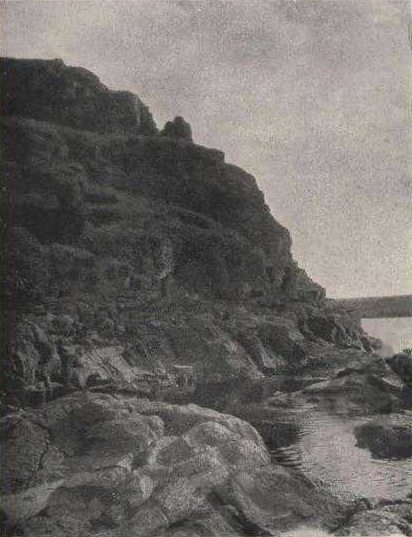
\includegraphics[width=0.85\linewidth]{chast-zmiy/ktotakiezmei/tav01.jpg}
\end{center}
\vspace*{\fill}

\newpage
\vspace*{\fill}
\begin{center}
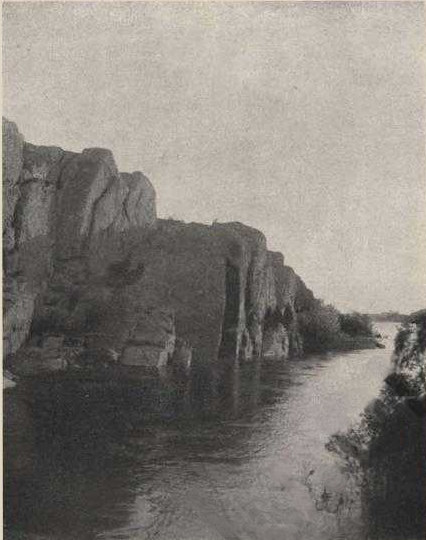
\includegraphics[width=\linewidth]{chast-zmiy/ktotakiezmei/tav03.jpg}

\textit{Таволжаный остров с востока, со стороны острова Перуна.}
\end{center}
\vspace*{\fill}
\newpage
\vspace*{\fill}
\begin{center}
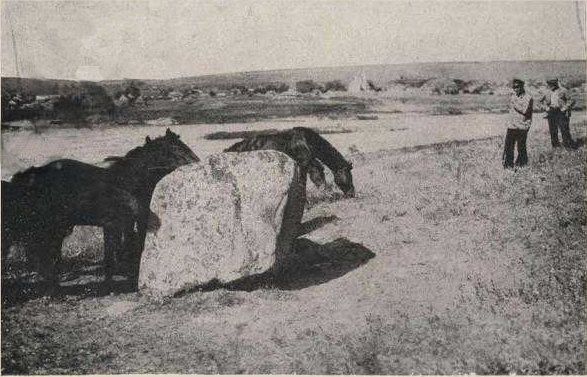
\includegraphics[width=\linewidth]{chast-zmiy/ktotakiezmei/tav02.jpg}

\textit{Таволжаный остров, Орлиная скала. Тут найдена была мастерская бронзового века.}
\end{center}


\begin{center}
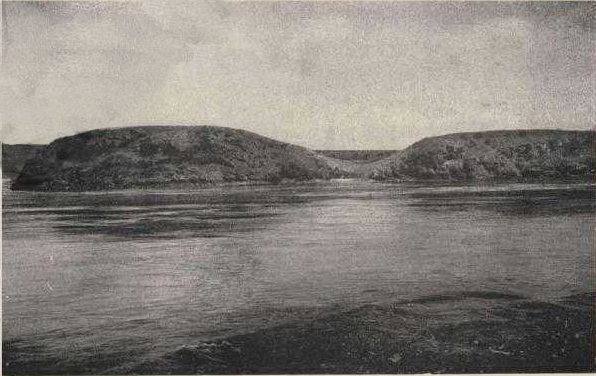
\includegraphics[width=\linewidth]{chast-zmiy/ktotakiezmei/per01.jpg}

\textit{Остров Перун до затопления.}
\end{center}
\vspace*{\fill}
\newpage
\vspace*{\fill}
\begin{center}
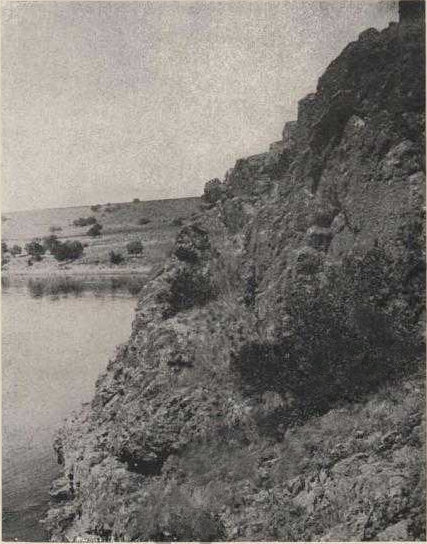
\includegraphics[width=\linewidth]{chast-zmiy/ktotakiezmei/per02.jpg}

\textit{Высшая скала Перуна.}
\end{center}
\vspace*{\fill}
\newpage

%Остров Перун до затопления:

%\begin{center}
%\includegraphics[width=\linewidth]{chast-zmiy/ktotakiezmei/o-perun-01.jpg}
%\end{center}

%\begin{center}
%\includegraphics[width=\linewidth]{chast-zmiy/ktotakiezmei/o-perun-02.jpg}
%\end{center}

%\newpage

%Тоже остров Перун:

%\begin{center}
%\includegraphics[width=\linewidth]{chast-zmiy/ktotakiezmei/o-perun-03.jpg}
%\end{center}

%\newpage

Приступим к изучению источников. Для удобства упорядочу их по времени публикации, что позволит сделать любопытные замечания. Боплан с его рассказом о Таволжаном острове будет процитирован к месту.

У Афанасьева-Чужбинского в «Поездке в Южную Россию. Очерки Днепра» (1861), составленной на материале его статей, напечатанных несколькими годами ранее в «Морском сборнике», я отыскал легенду о Змеиной скеле\cite[том VII, стр. 116]{afanchujb}, как еще называли остров Перун. Приведу что пишет Чужбинский:

\begin{quotation}
Пройдя Языкову, барка принимается за весла и огибает большой  остров Таволжаный (названный у Боплана Таволжаном), покрытый хорошею растительностью. Прошлый год мне рассказывали, что на этом острове есть глубокое озеро, и в нынешнюю поездку я отправился на Таволжаный. Действительно озеро существует в обрывистых берегах, и, как говорят, рыбное. В Языковой мне рассказывали, впрочем, что не далее как прежний владелец напускал туда рыбы и таким образом развел её. 

Огибая Таволжаный остров, барка делает усилие держаться ближе к его берегу, чтобы не зацепиться за Змеиную скелю. Это отдельный утес, брошенный в Днепр у самого левого берега и придающий местности какой-то дикий колорит. Название Змеиной скели всегда возбуждало мое любопытство, и прошлый год, плывя первый раз через пороги, я останавливался возле нее и лазил в пещеру, вход в которую в летнее время не залит водою. По рассказам лоцманов в этой скале жил когда-то змей, именно в описанной пещере, которая, будто бы, после разных изгибов выходит на верх утеса. В настоящее время она небольшая и весьма низкая.

Меня однако же не удовлетворило это весьма краткое и голое предание.

Прошлою осенью и нынешней весною, проживая на порогах, я продолжал мои расспросы как у лоцманов, так и у береговых жителей, и хотя собранные мною сведения тоже довольно бедны, однако все же дают некоторое понятие о том, что в прежние времена баснословные предания об этой скале имели размеры гораздо обширнее. 

Когда-то в ней жил змей-царь, у которого была дочь красавица. Змей о трех головах берег свою дочку, чтобы она не полюбила какого-нибудь русского царевича, и однако же не уберег, потому что красавица уплыла с каким-то витязем вниз по Днепру, в Черное море. С тех пор змей сделался свирепее и каждый день вылетал куда-нибудь в окрестность за новою жертвою.

Это предание древнее, а новейшие говорят, что на скале множество змей, длиннее обыкновенных, очень свирепых, и, будто бы, лет тридцать назад небезопасно было входить в пещеру, а тем более взбираться наверх.

Любопытство туриста заставило меня вскарабкаться на Змеиную скелю. Это было очень недавно, следовательно змеи могли бы разгуляться по своему владению, однако в течении получаса мы не встретили там ни одного пресмыкающегося.

Искал я и выхода знаменитой пещеры, но и того не оказалось. 

Есть два углубления, похожие на следы человеческого жилища, но это будет без всякого сомнения землянки каких-нибудь лугарей.
\end{quotation}
 
В 9 томе (за 1857 год) «Морского сборника» Чужбинский со страницы 19 (неофициальной части) пишет о другой Змиевой пещере, около села Волошского (жили там и Волохи, и Украинцы).

\begin{quotation}
Положение села чрезвычайно живописно, в особенности нижняя часть его часть, окружающая огромную отдельную скалу, упирающуюся с Севера в Лоханский порог и одетую с этой стороны больших размеров глыбами гранита. На самом верху тоже разбросаны громадные камни, и оттуда превосходный вид на оба порога и окрестности. Мне кажется, если бы красота видов села Волошского была известна, многие проезжающие сворачивали бы сюда из Екатеринослава нарочно для того, чтобы полюбоваться интересной местностью.

Кое-где по скале разбросаны небольшие курганчики, изрытые искателями кладов.

Южный бок этой скалы огибает овраг, на противоположной стороне которого высится такой же вышины гора, одетая гранитом. В последней, под одним камнем есть пещера, по словам местных жителей, проникающая в глубину саженей на десять. Говорят, что там ничего нет, но что очень сыро и холодно.

Бывая в Волошском, я хотел осмотреть эту пещеру, но проникнуть мог лишь аршина на два, а дальнейший вход засорен так, что требовалось бы много хлопот. В другое время эти хлопоты меня не испугали бы, он имея в виду совершенно другие занятие и тем более живя на порогах, я употреблял все свое время на плавание между камнями, в обществе рыбаков – местных лоцманов, что было мне необходимо для основательного изучения местности.

Об этой пещере рассказывают, что в ней жил когда-то змей, пожиравший людей – сказка, повторяющаяся во многих местах и, к сожалению, лишенная всяких подробностей.
\end{quotation}

Но вернемся к Перунову острову. Развею неточность. В сети можно прочитать, что «исследователи Одесского общества истории и древностей» в 1863 году нашли в Змиевой пещере на Перуне человеческие кости, и дается ссылка на 5-й том «Записок Одесского общества истории и древностей» (Одесса, 1863). На деле эти «исследователи» – перевод Д. Ч. Шершеневича с польского отрывка статьи Подберезского (корреспондента Общества), и напечатан оный в шестом томе, в 1867 году, под названием «Геркулесовы столбы на Днепре». 

Переводной Подберзский весьма много пересказывает работы Чужбинского, причем очень близко к подлинникам на русском. А толкование географии по Геродоту взято из статьи Н. Надеждина «Геродотова Скифия, объясненная чрез сличение с местностями» из первого тома Записок Одесского Общества Истории и Древностей (1844 год).

Подберзский пишет сразу про две змиевы пещеры:

\begin{quotation}
У третьего, по порядку, Лоханского порога, на правом берегу, расположена в долине деревня Волошская, известная красотою своего местоположения. Южною оконечностью своею она примыкает к огромной скале, входящей в порог и установленный, со стороны деревни, огромными торчащими обломками гранита. С ея вершины, также покрытой обломками камней, открывается прекрасный вид на соседний Сурский порог и на шумящий у подошвы ея Лоханский порог.

Южную сторону этой скалы опоясывает глубокий овраг, за которым поднимается другая скалистая гора. Там, под одним из камней находится пещера, идущая, как говорят, сажень на десять в глубину; но вход в нее завален камнями и никто не мог исследовать настоящей ея глубины.

По преданию, в этой пещере обитал змей, пожиравший людей. Вообще, если бы эта местность была тщательнее исследована, то может быть, нашлись бы какие нибудь древности, потому что это место, кажется, имело значение в древние времена, как свидетельствует об этом несколько курганов, стоящих на первой горе, и неизвестно кем разрытых. [...]\footnote{Следует исчисление и описание Порогов (подробности в третьем томе «Записок» на странице 581) – пропускаю.}

Держась постоянно левого берега, мы миновали большой остров Таволшан, простирающийся на три версты в длину, и известный у Боплана под тем же именем. В конце острова, вдается в Днепр нависшая скала, называемая Змеиною. В этой скале, под уровнем воды, видно узкое отверстие, вход в змеиную нору, засыпанный отчасти песком. Это отверстие внутри расширяется в обширную пещеру, в которой множество человеческих костей; из нее поднимается как бы крутой выход на вершину скалы, но он не был ни кем окончательно исследован.

Г. Чужбинский собрал рассеянные в народе остатки древнего предания (Морской Сборник за 1857-58 годы), из которого видно, будто бы в этой пещере обитал некогда Царь-Змей, у которого была красавица дочь. Змей этот был чудовище о трех головах; он стерег свою дочь, чтобы она не полюбила какого-нибудь Русского царевича; но это не помогло, потому что красавица полюбила чужеземного героя и бежала с ним тайно, по Днепру, к Черному морю. С этого времени жестокость змея усилилась, и он ежедневно выходил из пещеры искать между людьми новых жертв для своей мести. 
\end{quotation}

Остров Перун как название, не Змиева скеля, а именно Перун, после летописи появляется только в легендарной книге зачарованного казачеством ученого-этнографа Дмитрия Эварницкого (Яворницкого, 1855-1940) «Запорожье в остатках старины», вышедшей двумя томами в 1888 году. Яворницкий облазал и обплавал тот край вдоль и поперек, собирал предания, кроме прочего посещал и многочисленные пещеры.

Кстати именно с него Репин срисовал образ писаря для своего полотна «Запорожцы» (пишут письмо турецком султану). Лицо, руки – всё от Яворницкого. На второй, незавершенной, затрапезной версии «Запорожцев», которая хранится в Харьковском художественном музее, писарь еще более похож на своего живого подлинника. Как отличать варианты картины навскидку? На «харьковской» писарь в очках и смеется. Яворницкий снабжал Репина и запорожскими вещами – предметами одежды, курительными трубками и тому подобным.

\begin{center}
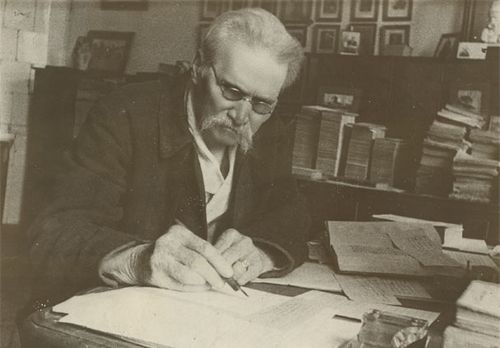
\includegraphics[width=\linewidth]{chast-zmiy/ktotakiezmei/yavornyckiy01.jpg}

\textit{Дмитрий Яворницкий.}
\end{center}

Плодом деятельности ученого стала написанная с вдохновением книга. В первом томе не обойдены вниманием острова Таволжан и Перун. Поскольку речь идет о вещах исчезнувших, а книга редкая и мало у кого дойдут до нее руки, помещаю важный текст Яворницкого почти целиком, выпуская лишь песню, имеющую отношение к растению таволге.

\begin{quotation}
Ниже Будиловского порога впадают в Днепр балки Трутова или Рединова с правой стороны, Будилка – с левой, на две версты ниже порога: за ними следуют камни Сазоновы, Колесники, балки Рябого, Канцеская, с правой стороны, камень Червоный, острова Червоный и Осокороватый, иначе Склуб или Рыбачий, против деревни Федоровки (Языковой) на правом берегу, камни Службы, балки Квитяна, Щербина, балка Куценька, у правого берега, выше деревни Августиновки (Сольщи), балки Калинова, Глодовы (две), камни Черево, Черевиня, забора Таволжанская, у Лерберга\footnote{Имеется в виду работа «Исследования, служащие к объяснению древней Русской истории» Лерберга, 1819 года. Лерберг в разделе о порогах пишет об острове Таволшанском: «между им и правым берегом, русло реки наполнено скалами; по левой стороне обтекает его Днепр, все еще имеющий большую ширину, а против южного конца его, там, где между им и левым берегом лежит узкий остров Пернов, находится десятый, но неважный порог, который по главному острову называется Таволшанским».} порог Таволжанский и наконец остров Таволжанский. В этом месте, по словам Эриха Ласоты, у татар была главная переправа через Днепр.

Остров Таволжанский, иначе Таволжанка, по местному произношению Тивильжан, известен был с этим же названием еще Эриху Ласоте, а вслед за ним и Гильому де-Боплану. 

«Второй остров\footnote {Это выдержка из «Описания Украины» Боплана, Спб., 1832, стр. 23. Боплан в публикации 1660 года насчитал всего два острова на порогах, не заливаемые весенней водой – первый это Стрельчий, и второй – Таволжаный.} (Таволжанский) гораздо более длиною около 2000, шириною около 150 шагов: он весь составлен из скалы, но не имеет столько утесов, как первый. Место это крепко от природы и хорошо для житья. Здесь растет много таволы: это – красное дерево, твердое как бук и имеющее силу гнать из лошадей урину. Из него выделывают краску для волос».

В настоящее время остров Таволжанский имеет в длину две версты, в ширину от десяти сажен до одной версты, по краям окаймлен лесом, а по середине представляет из себя прекрасную ровную площадь, по которой кое-где разбросаны огромные гранитные скалы, из коих самая высокая носит название Голубиной скели; с этой Голубиной скели открывается прекрасный и далекий вид на д. Августиновку (Смольщу), находящуюся у правого берега Днепра, против правого берега острова Таволжанки, и на самый Днепр, вдоль по направлению от юга к северу.

Видимо, название свое остров Таволжанка получил от растения «таволги», в большом обилии произрастающего на нем даже и в настоящее время. Таволгою (spirea) местные жители называют особый род красной, очень тонкой лозы, производящей жуткую боль, когда ею ударить себя. [...]

Ниже острова Таволжанского, у северного конца его\footnote{Как же ниже, если выше это на север?}, стоит остров Орлов\footnote{Сохранилось село Орловское (48°5'18"N 35°5'5"E), Волнянского района, почти примыкая к селу Перуну на запад. По переписи населения 2001, население Орловского 45 жителей, население Перуна – 32 человека.}, длины полтораста сажень, против него впадает в Днепр балка Орлова и за балкой Орловой балки Большая Бицулина, Малая Бицулина, Зализна, Гелеверина, потом следуют камень Тарань, балка Безкровная, с правой стороны, балка Таволжанка, с левой стороны, и против нее небольшой, но громкий остров Перун.

Перун, или, как называют его местные жители, П\'ерун или даже П\'ерен, расположен параллельно острову Таволжанскому, только у самого берега Днепра и как раз против балки Таволжанки, идущей к левому берегу Днепра и разделяющей самый остров на две половины; это разделение острова дает повод думать, что некогда он составлял одно целое с левым берегом реки и что на нем оканчивалось устье балки.

Остров протянулся вдоль левого берега Днепра, от севера к югу, причем в северной половине он далеко выше, чем в южной. Длина – сто пятьдесят сажен, ширина в северной окраине – семьдесят пять, в южной – тридцать сажен; высота, при среднем уровне воды в Днепре, в северной окраине – пятьдесят сажен, в южной – тридцать\footnote{Длина 320 метров, ширина в северной окраине 160 метров, в южной – 64 метра, высота, при среднем уровне воды, в северной окраине 106 метров, в южной 64 метра.}.

В общем о. Перун похож на огромное чудовище, протянувшееся по Днепру головой на север, хвостом на юг и посередине имеющее как бы перехват. По высоте – это единственный остров на всем Днепре.

На откосе западного берега Перуна есть пещера, носящая название Змиевой, похожая, впрочем, скорее на нору, естественную, чем на то, что мы называем пещерою, и имеющую длины восемь аршин, ширины, при входе в нее, полтора аршина и высоты, также при входе, до двух аршин\footnote{Длины 5,7 метра, ширины, при входе в нее, 1 метра и высоты, также при входе, до 1,4 метра.}.

Кроме пещеры, на острове, в лощине, разделяющей его на две половины, есть еще погреб, стены которого выложены гранитным камнем; длина его – пять сажен, ширина – три сажени\footnote{10,6 на 6,4 метра.}. Кто сделал этот погреб и для какой цели, указаний на это мы не имеем. Может быть, можно было бы сказать что-нибудь положительное на этот счет после раскопки погреба. Но, к сожалению, едва ли это можно сделать, так как он уже раскопан какими-то искателями клада.

Остров принадлежит двум владельцам: Н.\- П. Петренку, владельцу села Петровского, и С. П. Иваненковой, владелице села Андреевки. На вопрос, отчего остров Перун получил свое название, отвечают преданием, весьма сходным с тем, которое занесено на страницы нашей русской летописи о низвержении св. Владимиром идола бога Перуна, брошенного, по повелению князя, в Днепр.

«Как поплыл тот Перун по Днепру, так достиг до самого острова Тивильжана, тут же остановился и перекинулся в небольшой остров. Оттого там, где он лег головой, там самая большая высота на острове, а там, где он протянулся ногами, там самая меньшая высота на нем».

 – А почему вот та пещера, что в Перуне, называется Змиевой?

«А потому, что в ней жил змий, страшенный змий, – такой змий, что пожирал людей. Ухватит бывало какую-нибудь людину, притащит в пещеру да там и сожрет. От этого-то змия и пещера стала называться Змиевой. Это давно было, очень давно, еще не за нашу память, да и не за память, вероятно, наших дедов и прадедов».

Расположение двух островов параллельно один другому, в виде естественных плотин, было причиной того, что этом месте уже в очень давнее время существовала переправа через Днепр, как об этом свидетельствует Эрих Ласота.

«В настоящее время тут главная переправа даже за остров Таволжанский (Tawol-Zani), так как Днепр в этом месте не разветвляется и не очень широк»\cite[стр. 29]{lasota}.

[...]

Ниже Таволжанского острова идут: камень Ревун, против о. Перуна.
\end{quotation}

Из статьи Владимира Данилова «Отзвук былины о змееборстве Добрыни Никитича в украинским фольклоре» (Киевская старина, том XC, 1905 год) я узнал про несколько преданий, помещенных археологом и этнографом Яковом Павловичем Новицким (1847-1925) в статье «С берегов Днепра», напечатанной в изданном к XIII археологическому съезду в Екатеринославе «Сборнике статей Екатеринославского Научного Общества по изучению края». 

Тщетно пытался я разыскать сей сборник. Но к счастью, уже в нашем веке стараниями многочисленных институтов, товариществ и академий был выпущен пятитомник работ Новицкого\cite{novickiy01}, где во втором томе собраны почти все фольклорные прозаические записи ученого, относящиеся к Запорожью. Записи подверглись некоторой правке. Ведь Новицкий записывал украинскую речь, пользуясь русским алфавитом. При издании, тексты «перевели» снова на украинский. Сравнивая их с цитатами в статье Данилова отмечу, что искажений вроде нет.

Поэтому здесь и далее буду пользоваться вторым томом Новицкого как обильным источником легенд и бывальщин. 

\begin{center}
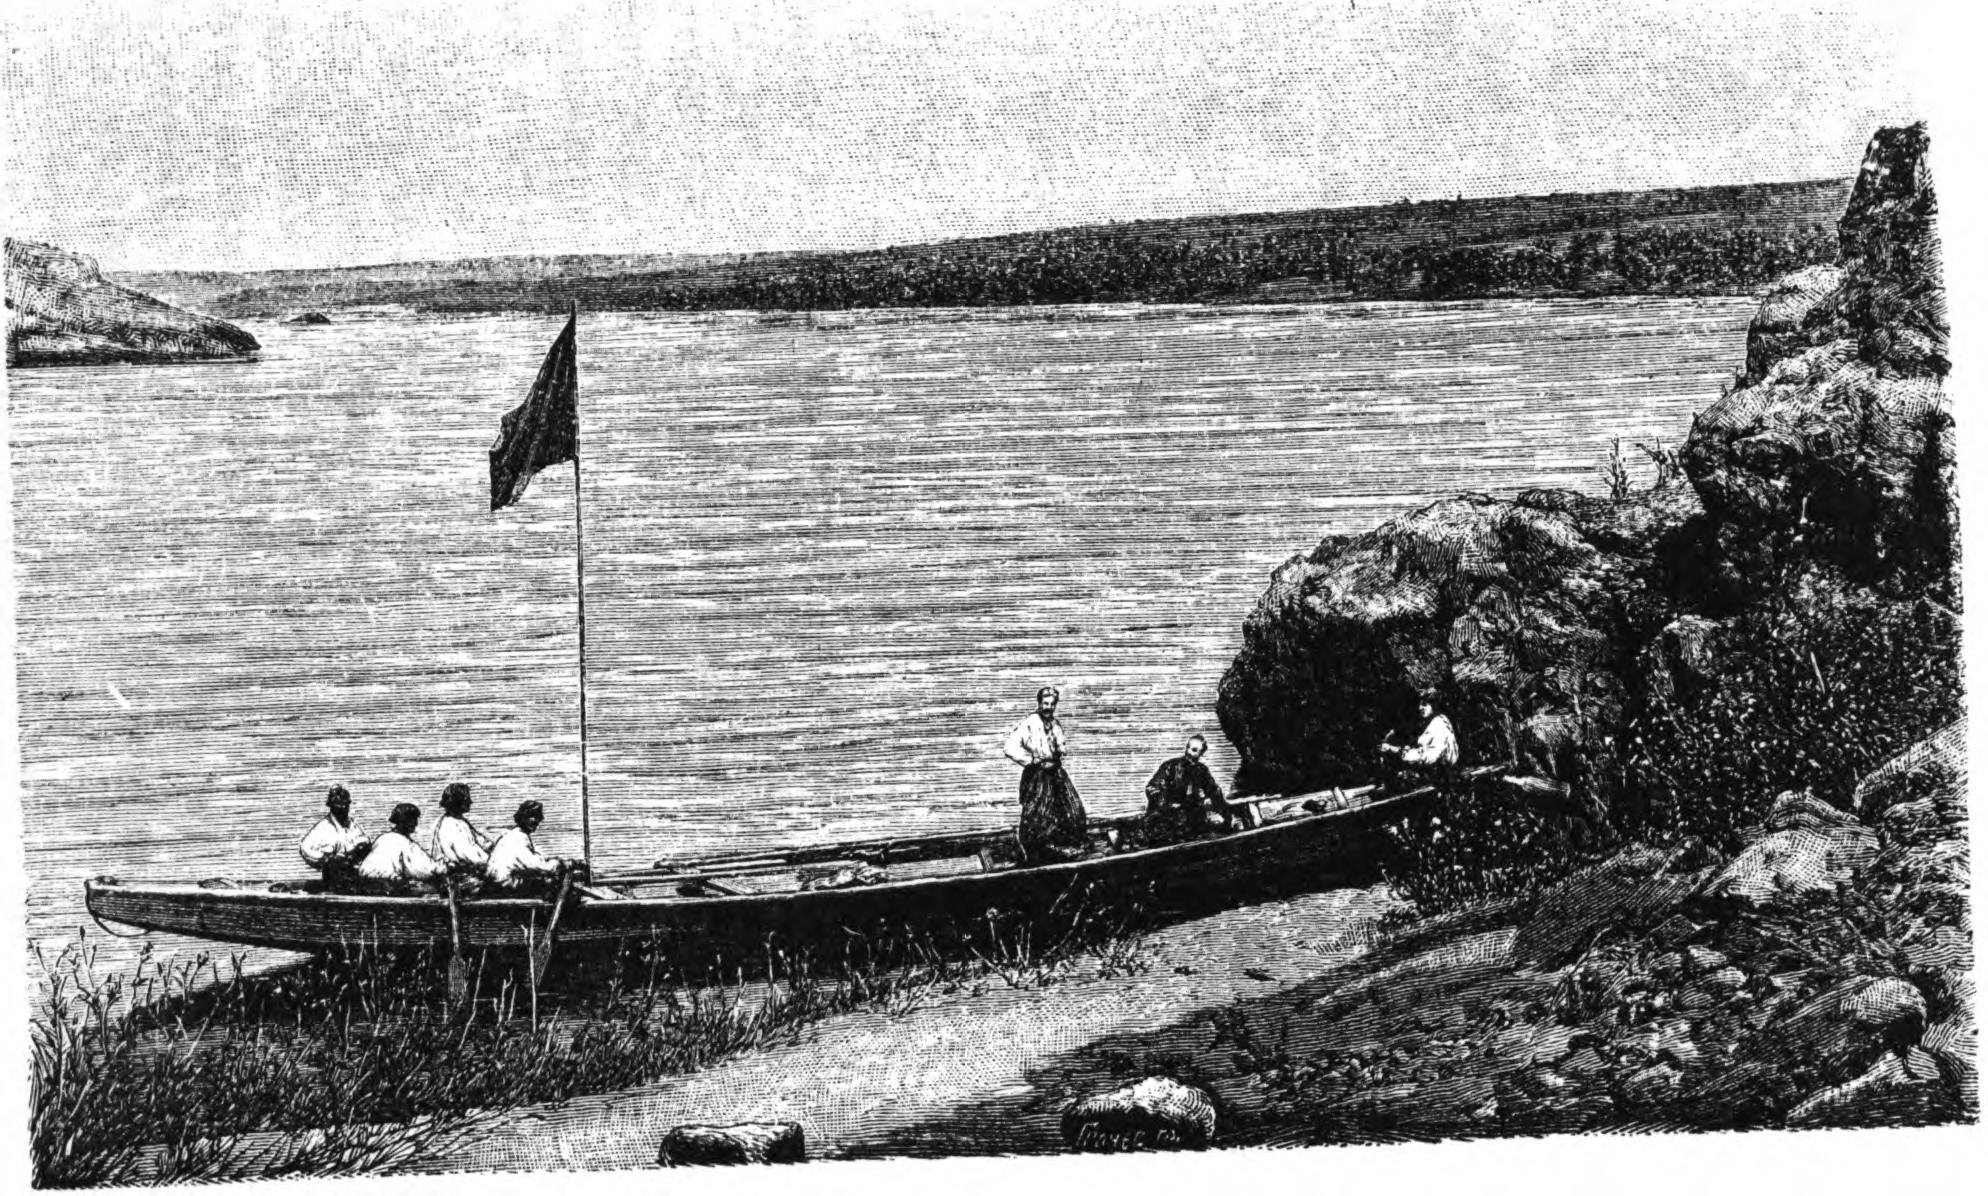
\includegraphics[width=\linewidth]{chast-zmiy/ktotakiezmei/Evarnickij_D_I_Zaporozhje.jpg}

\textit{«Камень Перун» – иллюстрация из книги Эварницкого «Запорожье...» 1888 г.}
\end{center}

Давайте почитаем сохраненные Новицким предания. Обратите внимание на постоянное использование слова «змий» применительно к идолу Перуну.

\begin{quotation}
Колись, кажуть, змій був на небі і літав по всьому світу; його всі боялись, а інчі і кланялись йому. Як узнав Бог, шо йому поклоняются, взяв і пооднімав крильця. Він упав з неба в Дніпро і поплів. Ідолопоклонці бігли берегом і кричали: «Перуне, Перуне, пріплеви до берега»! Преплів він до острова, і показалась йому глибока нора; він туди і пропав. Від того часу прозвано і острів Перуновим.

Дед Тимош Драган, 93 года, село Аврамовка Екатеринославского уезда, 11 апреля 1890 года.
\end{quotation}

\begin{center}
***\end{center}

\begin{quotation}
Кажуть, шо Перунового острівка тут не було, а преплив на йому змій відкільсь згори\footnote{То бишь откуда-то выше по течению.}. Як плів він, тоді б то, кажуть, однім боком бігли ідолопоклонці і виклікали на берег, а другім вийшли назустрічь православни і почали молебствовать і заклинать. Де стояли наші с корогвами, туда він підплів і став. – Змієва нора збоку – от Дніпра; вона, кажуть, була дуже глибока, та після того, як змій згінув – скеля зійшлася щільно, і нори нема. Буть то так було, а чи правда цьому, не знаю.

Дед Олексей Курта, 76 лет, село Смольща
Екатеринославського уезда, 12 апреля 1890 года.
\end{quotation}

\begin{center}
***\end{center}

\begin{quotation}
Нізче трохі Орлового, – острівок Перун. Про цей острів ось що чув я від старих людей. Якийсь то, кажуть, бог Перун плів Дніпром, і його хвилею викинуло на острів; тут його заховано, а потім откопано. На йому, кажуть, було золота 3 пуда, а сам зробленний з дерева. Від того і острів став Перун. На Перуні, від Дніпра, єсть нора: колись, кажуть, жів там змій, і йому носили людей. Нору звалі Змієвою.

Дед Михайло Кнырик, 96 лет, село Языково Екатеринославского уезда, 3 июня 1886 года.
\end{quotation}

\begin{center}
***\end{center}

\begin{quotation}
Стіко впамьятку – острів зветься Перуном. На йому висока скала, а в ній від Дніпрового ходу, – скота\footnote{«Скота» значит «пещера».}. До Христового рожденія, кажуть, жив там змій; він гарбав під себе жінок і дівок, а мужей пожирав. Як Христос народився – змія прокляв, а потім звоював його якийсь богатирь. У змія було, кажуть, три голови і крила. Він як летить – освіщає весь світ, а огонь так і палає.

На Перуні єсть клад. Як був я ще парубком, у нас в слободі жив такий старий дід, шо аж мохом поріс; йому було більше ста год, а звали Степаном Лисим. Це чоловік був ще запорожського званія. Він все, було, розсказує про клад на Перуні, тіко, казав, його страшно брать – заклятий. Про преміту казав так: від голови єсть лощина, а в лощині кущ жостіру, отступи від того куща три ступні на полудень і копай: там запорожці сховали каюк грошей і прикрили шкурою. Каюк, казав, такий, шо чоловік десять переїде через Дніпро.

Дед Лукиян Сотченко, 88 лет, село Петровское Свистуново, 13 января 1885 года.
\end{quotation}

В преддверии запуска Днепрогэса, а это 1927-1932 годы, когда многие земли Запорожья обречены были навсегда скрыться под водой, Дмитрий Яворницкий возглавил археологическую экспедицию, чтобы спасти для истории различные предметы старины. 

Были сделаны также фотографии и зарисовки мест – всё это лежит где-то в закромах, лишь время от времени извлекаясь для выставок. 

По итогам исследований, а также снимкам, сделанным ранее на субботних прогулках Яворницкого и его компании, в 1928 году вышел альбом фотографий с географическим очерком «Днепровские пороги» – его переиздали в 2002-м – оба издания редко где сыщешь, в электронном виде есть лишь текст и с дюжину сканов иллюстраций. У букинистов книга 1928 года стоит баснословные деньги.

В «Порогах» дано обстоятельное описание острова Перуна. На первый взгляд цельное, при внимательном прочтении оно распадается на составляющие. 

Так, начало похоже на переработанный текст из «Запорожья в остатках старины». Предания об острове и змее-Перуне, начиная со второго по счету, взяты у Новицкого, причем в той же последовательности, а первое предание у Яворницкого – из записей Афанасьева-Чужбинского. При этом Яворницкий, стремясь сгладить шероховатость народной речи, искажает смысл. Так, у Новицкого «якийсь бог Перун», то есть рассказчик не знает толком, что за бог такой, а в пересказе Яворницкого бог Перун вполне привычен, «якийсь» же стало «якось» применительно ко времени действия.

Сравнивая описание острова в «Запорожье» и «Порогах», видно, что в новой книге сочинитель увеличил количество используемых источников, свел их в ладное повествование и вложил записанные Чужбинским и Новицким предания в уста столетних дедов-старожилов. Поскольку мы уже знакомы с этими историями в исходниках, при цитировании их опускаю. И да простит меня Яворницкий за разрушение красивой целостности!

\begin{quotation}
Нижче Орлового острова підходять до Дніпра з лівого боку одна за одною балки: Велика Бицулина, Мала Бицулина і Таволжанка, і тут же впадає в очі невеликий, але дуже високий, скелястий, славний своєю назвою острів Перун, за місцевою вимовою Перун, навіть Перен. [...]\footnote{Пропускаю пересказ летописи и переделанный текст из «Запорожья» о том, что остров похож на чудовище.}

Можна думати, що в давню давнину цього острова зовсім не було, а була висока прибережна скеля, яка дуже висовувалась у лівий берег Дніпра. В одну велику весняну повідь дужий навал води, дійшовши до високої кам'яної прибережної скелі і не мігши зрушити її з місця, з страшною силою одкинувсь од неї ліворуч, розмив поза скелею землю й зробив острів Перун, так само, як це зробила велика вода й нижче, де з'явився острів Велика Хортиця.

Всієї площі землі острова Перуна 7 дес. Ост\-рів має 296 саж. довжини, 80 саж. ширини, 50–60 ф. у середній частині своїй і 98 ф. у вищій частині «голови» височини, при повному спаді води в Дніпрі\footnote{Яворницкий в обмере смешивает футы и сажени, перевожу на метры. Длина 631 метров, ширина 170 метров, высота 15-18 метров в средней части, 29 в наивысшей части «головы». То есть длина почти как в Киеве мост метро от ст.м. «Днепр» до берега Гидропарка.}. Перун вище Стрільчої скелі, що коло Лоханського порога, яка має 30 ф., але нижче сусіднього острова Таволжаного (150–200 ф.) і острова Великої Хортиці (300 ф.)\footnote{Лоханский: 9 метров, Таволжаный: 46-61 метр, Большая Хортица: 91 метр.}.

З західньої сторони острів Перун має печеру, яка зветься Змієва і в яку можна влізти тільки в липні місяці або в серпні, як вода в Дніпрі стоїть низько. Вона має в середині 7,5 арш. завдовжки, 1–1,5 арш. завширшки і 1,5 арш. заввишки;\footnote{Длина: 5,3 метра, и метр на метр в ширину и высоту.} кінчається вузькою ущелиною, яка піднімається вгору; з весни й до середини літа печеру заливає вода.

Року 1867 про цю печеру писав польський археолог Підберезький так: «У цій скелі (тобто Перуні) під рівнем води видно вузьку щілину, вхід в зміїну нору, почасти засипану піском. Ця щілина в середині розширяється у велику печеру, в якій дуже багато людських кісток; з неї начебто піднімається крутий вихід на верховину скелі, але його ніхто не досліджував».

Через ту Змієву печеру на деяких планах порожистої частини Дніпра та в деяких дослідувачів острів Перун неправильно називають «Змеиною скалою». У лоцманів і місцевих селян – це острів Перун.

Цей острів добре й гаразд знають старі лоцмани, які доводять, що колись на ньому був чудовий, розкішний, великий, густий ліс: росли вікові дуби, татарські кленки, гнучкі високі лози, густий глід; водились могутні орли, страшні окаті пугачі, дикі кабани, дикі кози, а між ними велика сила гадюк. Од дубів тепер лишились тільки пеньки, а од великих гадюк в розколинах скель дрібна гадючня.

На острові Перуні жили й запорожці, які добували тут так звану слюду (лисняк), що заміняла їм скло. Од запорожців, кажуть, тут лишився й льох, викопаний якраз посередині острова в так званій перепоясці. Кажуть, що в тому льосі запорожці закопали цілий каюк грошей; такий каюк, що в ньому десять чоловіка перепливуть через Дніпро. Щороку в тому льосі кладомани шукають гроші, але й досі не чути, щоб хто находив їх там. Учені люди находили тільки черепки од посуду неолітичного періоду кам'яного віку, та й то поки що не так багато. Про те, чому печера й самий острів Перун прозвали Змієвими, є декілька народних легенд. [...]\footnote{Мы уже ознакомились с ними по другим источникам.}

Супроти середини Перуна, на 16 саж. од правого берега острова, лежить у воді камінь Ревун, на «Атласе части реки Днепра 1863 года» – Реут, на «Карте Генерального Штаба» 1875 року – Ревун.

Коли виміряли зимою 1890 року 3 грудня цей камінь Ревун, то верховина його мала 5 ф., довжина – 6 саж. 2 арш., ширина – 5 саж., навкруги – 18 саж. В тиху літню ніч перед зміною години, кажуть, шум Ревуна переходить у глухий стогін, іноді в оглушливий рев, у шум з дзвоном, і тоді його чути далеко-далеко. Коли влітку поглянути на його білі вічноклекочучі хвилі, то здається, начебто стадо баранців скаче або руна шерсти, які підкидають угору. «Ревун кипить, наче в сукновальні сукно перевертається». Через те місцеві селяни на своїй мові звуть камінь Ревун Сукновальнею.
\end{quotation}

В «Порогах» Яворницкого и про остров Таволжаный рассказано куда более, чем в «Запорожье» – сообщается об остатках землянок на нем, двух курганах (один обложен вокруг гранитом) и находках кремневых ножей, черепков с орнаментом, форм для бронзового литья.

О пещере около села Волошского Яворницкий в «Порогах» пишет, попутно сообщая еще о нескольких близлежащих пещерах:

\begin{quotation}
Південна частина села Волоського кінчається високою кам'яною грядою. Там є дві високі гори; одна з тих гір зветься просто Скелею, а друга – Бичковою скелею. Вулиці й хати кінця села містяться в цьому межигір'ї. На підгір'ї Бичкової скелі, на землі колишнього селянина Якова Заскоки, єсть так звана Змієва печера. Печера та з дуже вузьким входом і, щоб пролізти в її середину, треба спершу проповзти два сажні животом по вогкій землі, витягнувши вперед себе руки, а потім того вже можна стати і йти ногами.

Скільки та печера має довжини, напевне невідомо: одні кажуть – не більше як 25 саж., а інші кажуть, буцімто вона тягнеться більше ніж на верству, і де саме її кінець, ніхто того не знає, бо ніхто не доходив до її краю. В одному місці печери, кажуть, є така глибока ямина, що коли туди кинути камінь, то не чутно, як він і на дно падає. На жаль, усього цього перевірити не можна, бо в селі, якраз коло печери, лупили камінь і завалили вхід у печеру камінням, груддям та землею.

На другому боці межигір'я, на так званій Коршуновій леваді, на крутому схилі скелі є ще декілька печер. У деяких вхід теж такий же вузький, що пролізти в них ніяк не можна, хоча й видко, що далі вхід ширшає. У дворі селянина Борща є печера, яка має 10-12 саж. завдовжки.
\end{quotation}

В другом месте книги Яворницкий упоминает еще один остров с пещерой – «убежищем змея»:

\begin{quotation}
Проти забори Явленої стоять серед Дніпра Пурисові острови. Пурисових островів звичайно чотири, малої води – вісім і більш: «їх-тут багато: один поверх одного». На «Плане части реки Днепра» 1780 року найбільший з цих островів зветься Куряків, а найменші – Мадишевськими островами. Віце-адмірал Пущін на «Атласе Днепра» 1784 року, академик Лерберг та дослідувач Бухтієв найбільший з островів називають Малим Дубовим. На «Топографической Карте Генерального Штаба» цей острів поставлений не на своєму місці й зазначений дуже малим. Прибережні люди звуть цей острів Прусовим, Явленим (од забори Явленої), Німецьким; меноніти колонії Кронсвайд називають його Дубовим або просто «островом»; у лоцманів він зветься Пурисів, як і всі менші теж Пурисові.

На першому од порога з цих островів є печера в скелі – «притулище змія».
\end{quotation}

На этих же Пурисовых островах найдено множество человеческих костей и оружия, как огнестрельного, так и сабель. Яворницкий цитирует Новицкого за 1905 год:

\begin{quotation}
Вступивши на найближчу до порога частину острова, ми зразу натрапили на розмитий весняною повіддю яр, на саженній глибині якого між камінням розкидані людські кості та зрідка черепки товстого глиняного посуду. Яр той тягнувся приблизно на 40-50 саж. Далі, оглядаючи піскові кручі яру, ми побачили цілу силу кісток: тут з-під піску обголились ребра, хребтові кістки, черепи й таке інше. Далі в однім місці, над кручею, натрапили на кущ шелюга, між корінням якого ховався цілий ворох кісток. Ми зробили розкопи в деяких місцях і знайшли в однім місці самі кістяки без голів, в другому – самі черепи з нижніми щелепами без шийних кісток, в третьому – окремі частини кістяків. Все це наводить на думку про колишнє страшне в цьому місці побоїще. Через те острів Пурисів дуже інтересний для наукових дослідів історика, археолога, антрополога. Про цю страшну людську могилу народ багато говорить, отже, і наука повинна сказати своє слово. Що це? 
\end{quotation}

Про Пурисовы острова, тамошнего змея, равно как и других змеев в том краю, Новицкий записал несколько преданий. Помимо прежних исследований своих, в 1904-1908 годах он провел раскопки на Хортице и её окрестностях на правом берегу Днепра, да издал книгу «Остров Хортица на Днепре, его природа, история и древности», где привел отрывками свои полевые записи.

О Змиевой пещере острова Хортицы есть такое: 

\begin{quotation}
В народной памяти много местных преданий, много легенд отмечено об острове Хортице и его урочищах, о Змеевой пещере. По сказаниям деда Фоки Горянца, после Христова Рождения, в пещере этой жил трехголовый Царь Змей, совершавший налеты на чужие страны и вступавший в битву с богатырями велитнями (великанами). 

По сказаниям деда Степана Штепы, здесь, как и во всем Поднепровье, жили великаны, жили богатыри, жили, наконец, трехголовые Змеи... Брошенные у берегов и среди Днепра Скалы – это дело богатырской потехи; сохранившиеся в скалах пещеры – это логовище чудовищных Змеев...

По рассказам 84 летнего рыбака Осипа Шутя, скоротавшего остаток лет на Хортице, остров этот знают старые люди всюду. В молодые годы бывал он в Донщине, за Кубанью, в Черноморье, на рыбных косах Азовского моря, и куда его не бросала судьба, везде находил старых земляков, везде спрашивали его, что сталось с Хортицей, с порогами Днепра; живут ли там потомки запорожцев...

В Черноморье седой старик спросил его: «Живет ли и поныне на Хортице Змей с тремя головами?». И когда он ответил «нет», старик, покачав головою, заметил: «Правду кажеш, козаче: помандрував він слідком за запорожцями в Туреччину, звалував за ними і звір всякий»... Дед Осип, передавая рассказы о Змеях богатырях, поясняет, что «во всем Запорожье жило три змея, из них один на острове Хортице, другой на острове Пурисовом, ниже порога Гадючего, где есть пещера, а третий, самый чудовищный и лютый Царь Змей, – Змей – над Змеями, – на острове Перун. Последний, говорят, имел два логовища: на Перуне и Стрельчьей скале, что близ порога Лохана. Все эти три Змея, летая по ночам, искрами крыльев освещали пороги и ночной путь запорожцев... Змеи жили как богатыри и вступали в битву только с богатырями. Они охотились на людей, одних только запорожцев не трогали, так как и между ними были богатыри и характерники»...
\end{quotation}

И всё равно Змей с острова Перуна – самый главный! Отметим сходное поведение всех троих – летают по ночам, искрами крыльев освещают пороги. «Жили как богатыри и вступали в битву только с богатырями» – точно как в былинах, которые мы скоро подробно разберем.

А вот чему очевидцем был в 16 веке неведомый создатель «Казанского летописца» – возможно, священник Иоанн Глазатый, проведший 20 лет в плену у татар. Он пишет\cite[стр. 67]{kazanletop}:

\begin{quotation}
О бесе, о творящем мечты пред человеки, живуще во градце.

К сему же третие знамение при мне же бысть, еще бо ми тогда в Казани живуща. Бе не в коем улусе Казанском мал градец пуст, на брезе высоце Камы реки стоя, его же Русь имянует бесовское градищо, в нем же живяще бес, мечты творя от много лет.

И то бе еще старых Болгар молбище жертвенное. И зхожахуся ту людие мнози со всея земли Казанския, варвры и Чемериса, мужи и жены, жрюще бесу и о полезне себе вопрошаху от ту сущих волхвов\footnote{Итак, в заброшенном городке жили бес и волхвы, и туда сходились язычники для принесения жертв.}. 

Бес же аки овех от недуг исцеляше, овех, с нерадением минующих его, уморяше, не пометнуших ему ничто же и плавающих рекою опроверзаше лади, потопляше в реце\footnote{Одних бес исцелял, а кто ему не молился, уморял, и перекидывал ладьи тех, что не жертвовали ему, проплывая мимо рекою.}, – чюдо же, от христьян неких погубляше.

Тем никто же не смея проехати его не поверхши мало что от рухла своего, и к вопрошающим ответ невидимо отдаяше жерцы своими, комуждо их долголествие сказываше, смерть и здравъе, и помощь, убытцы и на землю их пленение и пагубу, и всяку скорбь\footnote{Поэтому никто не смел проехать, ничего бесу не пожертвовав, а тот невидимо давал ответ, прочество.}.

И на воину пошедше жряху ему совопрошающися с волхвы, аще з добытком или с четою возвратятся; бес же проявляше им впред и сим прелщаше, овогда же и яша\footnote{Шедшие на войну тоже жертвовали и через волхвов получали ответ, вернутся ли с добычей.}.

И посла тогда царь самого Сеита Казанского вопрошати, аще одолеет Казань Московский царь, князь великий или Казанцы ему одолеют, и до 10 дней павше кляцаху на землю молящеся ерея бесовския, не востающи от места и мало ядуще, да не умрут з гладу\footnote{Казанский царь послал Сеита вопросить волхвов, иереев бесовских, и те 10 дней камлали, валяясь на земле и почти не кушая.}.

Минув 10 днеи, в полудни отозвался глас от беса в мечте, глаголюще, всем людям слышащим: «что стужасте о мне? Уже бо вам отныне несть на мя надежи, ни помощи ни мало от мене, отхожю бо от вас в пустыя места, непроходная, прогнан Христовою силою; приходит бо сюда со славою своею, хощет воцаритися в земли сеи и просветити святым крещением»\footnote{Прошло 10 дней, в полдень в мечети отозвался бес, так, что все слышали. Говорит – чего зовете? Не будет от меня больше помощи, ухожу, прогнан Христовою силою.}.

И по мале часе явися дым черн, велик, изнутри градца, из мечети, на воздух идя, смрад зол, из дыма же излете змий велик, огнен, и на запад полете, всем нам зрящим и чудящимся, и невидим бысть изо очию нашею. И разумеше вси бывшее ту, яко исчезе живот их.
\end{quotation}

Эта впечатляющая концовка со стартом беса из мечети и последующим его полетом, не только описывает проявление некой технологии полёта, летательного аппарата, но сильно напоминает полеты запорожских змиев. Будучи свидетелем явления, летописец точно передал его словами. 

Из дыма при запуске – змий огнен. И дальше на запад.

Кстати сама Казань, по преданию, стоит на месте змиева логова, там жил змей, у которого одна голова была воловья – ею он пожирал людей, а другая – змеиная, она питалась травой.
   
Змеи о нескольких головах, как мы помним, жили и на днепровских порогах. Снова нам пригодятся этнографические записи Якова Новицкого.

\begin{quotation}
В старі годи, по бальці Гадючій, був густий дубовий ліс і скрізь понад балкою росли груші і кислиці. В бальці стіко водилось гаду, шо страшно було і ходить. Восени, тоді саме, як гад поховається в нори, ходемо, було, по груші і кислиці. Отсе, було, як прогорнеш листя під деревом, то так і нагребеш мішок груш. Та ще й груші не які небудь: мнякі та добрі.

Ще, кажуть, в Гадючій бальці водились полози, а низче порога Гадючого, на острівку, була, та і теперь єсть – скота, де жив Змій с трьома головами; його всі боялись... Оце як летить, то так весь світ і засяє! Це було давно.

Зміїв, кажуть, водилось тут три: один на Перуні, другий на Гадючому порозі, третій – на острові Хортиці. 

На Хортиці, якраз в Висчій Голові, єсть і тепер глибока скота; ми її так Змієвою і звемо. Супротів остріва Пурисового, шо низче порога Гадючого, покопані городки\footnote{Редуты.}, де, кажуть, война була, а ще низче, де Старий Кронцвей, скрізь по піску багато невеличкіх могилок; вони всі мов обкладені камінням. Як був я малим і пас німецьку череду, то було часто находю мідні стрілочки: після великого вітру або після дощу, так і лежать, було, поверх піску.

Дед Фока Горянець, 71 год, село Вознесенка Александровского уезда Екатеринославськой губернии. 10 августа 1886 года.
\end{quotation}

Значит, змий с островка ниже Гадючей балки был трехголовым, обитал в пещере, и когда летел, то весь мир аж сиял.

А вот об одной из Змиевых пещер – Новицкий не указывает, какой именно:

\begin{quotation}
 – А отчего, диду, пещера названа Змиевою?

 – Колись тут жив змій.

 – Что же это такое за змей был?

 – Страшенний!.. Було у його три голови і один хвіст... Він літав і пожірав людей.

 – А давно його не стало?

 – Цього гаразд не докажу... Мабудь, ще тоді, як запорожці воювали нагайву та татарву. Це була земля турецька.

 – Откуда же пришли эти запорожцы воевать татарву?

 – І цього не докажу. Розсказують тіко, шо народ був отчаяний, здоровий.
\end{quotation}

Этот змей тоже летает и жрет людей. Змеи всё время летают. А для полетов, как известно, нужен керосин. И это есть.

Новицкий записал любопытный вариант известной легенды про Козьму, Демьяна и змия:

\begin{quotation}
Колись на землі жив змій. Багато він пожрав людей, – бо дужчого його на світі не було. В те времья жили Кузьма і Демьян, – божі ковалі.

От задумали вони того змія з світа згубить. Змій сунувся до їх, а вони – в кузню і заперли залізні двері. Змій і каже:

   – Кузьма Демьян, божі ковалі, відчиніть, а то ковтну вас с кузнею...

Ті і одвічають:

   – Коли ти силу маєш, пролижі двері: сядемо на їзик і ковтай.

Змій лиже, та й лиже, а святі гріють та й гріють залізо та кують клещі.

Пролизав змій двері, всунув язик. Кузьма та Демьян клещами за той язик і почали гатить молотами... Уморили змія, запрягли в плуг, шо на дванадцять пар волів, і давай орать. Орали степ вздовш, орали впоперек, і стілко змій не просив – не давали йому ні пити, ні їсти.

   – Буде с тебе, – кажуть, – і того жиру, шо откохався на людях...

   – Ну, – каже змій, – коли так, то перед Страшним Судом освітю я своїм жиром весь світ...

Чи довго ще орали, чи ні, – дійшли до моря. Змій – в море і давай згарячу пить... Пив, пив, випив все море і лопнув... Кузьма Демьян взяли і закопали того змія під горою. Бог його зна, коли це в світі було, а ось
небагато годів, як полився гас\footnote{«Гасом» называли керосин.} с тієї гори. Це б то і кінець світа близько...

В слободах і тепер не всякий світе гасом, бо він нечистий. Так от, коли хочете знать, відкіля взялися по степах річки і балки! Кузьма та Демьян поки не заморили змія, – орали глибоко – і потекли річки, а як заморили, орали мілко – і стали балки.

Дед Григорий Омельченко, 80 лет, полтавец, село Крестовка Мариупольського уезда Екатеринославськой губернии, 16 мая 1905 года.
\end{quotation}

Из той горы, где закопали змея, стал сочиться керосин. Наш современник может подумать, что у змия пробиты топливные баки.

В другой быличке речь идет о мирном, но тоже летучем и освещающем окрестности змие из Змиевой пещеры в Верхней голове – это северная часть Хортицы:

\begin{quotation}
Були жовтобрюхи, полози, а в пещері, шо в Вищій Голові острова Хортиці, кажуть, жив Змій. Він нікого не займав і козаки його не боялись.

Було, кажуть, вночі змій як засяє, як засяє – так і освіте Дніпро. 

Він, кажуть, не щоночі і показувався, а так в місяць або неділі в три раз і все біля пещери, шо і тепер звемо Змієвою. 

Як подались відціль запорожці під турка, пішла за ними риба і птиця, звалував і звірь всякий... Після того, кажуть, як зійшли запорожці, тут, по скелях, щось ходило і тужило... Було вночі як заголосе, так аж тіло холоне... А потім с Кічкасского боку як почне кидать каміння на Хортицю, як почне, то так те каміння і прикіпа на Чорній скелі... Сумно і страшно було тоді...

Дед Йосип Шуть, баштан на острове Хортице, 16 августа 1887 года.
\end{quotation}

Возможно, «змеи» имели небольшие летательные аппараты, различные части которых и принимались за несколько голов, хвосты, хоботы и тому подобное. С точки зрения современных знаний, предполагаю, что это было нечто вроде заплечных реактивных ранцев с крыльями.

С древних времен в городищах и курганах сохранились металлические и костяные фигурки человекоподобных существ в заплечных летательных аппаратах. Хорошо известны такие находки в Сибири, на Урале. Коренные жители считали, что это фигурки богов, а создателями фигурок называли предшествующее население, давний «волшебный» народ – чудь белоглазую. В преданиях, чудь по признакам сходна с эльфами – обладая умениями, превосходящими человеческие, они вроде ушли то ли внутрь холмов, то ли в другой мир. Этот переход мне неясен. Ведь говорят о нём люди, и – путано.

Есть хорошая подборка иллюстраций в книге «К истории искусств и верований у приуральской чуди, чудския изображения летящих птиц и мифических существ» Анучина\cite{anuchin01}. Там приведены и другие фигурки – гуманоиды верхом на огромных ящерах, свидетельство былой действительности. Покажу их также. Всё называю своими именами, как я трактую, без лишних осторожностей – мол, а вот удивительно похоже на! Не удивительно похоже, а так и есть!

\begin{center}
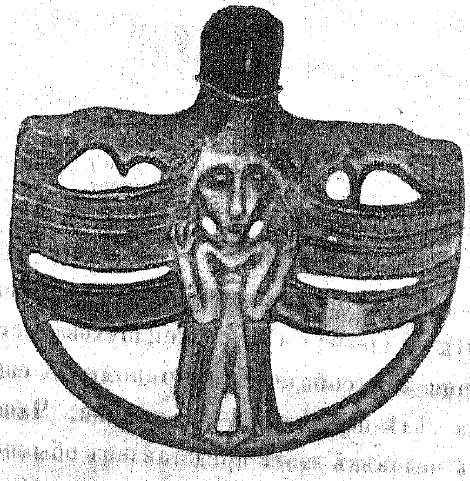
\includegraphics[width=0.60\linewidth]{chast-zmiy/ktotakiezmei/ural-bogi-10.jpg}
\end{center}

Фигура в заплечном летательном аппарате. На голове шлем. Руками пилот держится изнутри за крылья, нижний полукруг служит частью каркаса. Крылья состоят из пластин, которые подобно вееру складываются друг в друга в сторону верхней части, при необходимости сдвигаясь вниз, раскладываясь в полукруглой раме и создавая крыло с нужной площадью поверхности. Выступ над головой пилота встречается на множестве других подобных устройств. Это бак с топливом или турбина авиационного двигателя. 

А вот отдельная голова, тоже в шлеме, причем напоминающем велосипедный. Такой шлем очень легкий, для облегчения верх делают не сплошным, а в виде рамы. Вес наверняка имел значение и для летательных аппаратов «змеев». 

\begin{center}
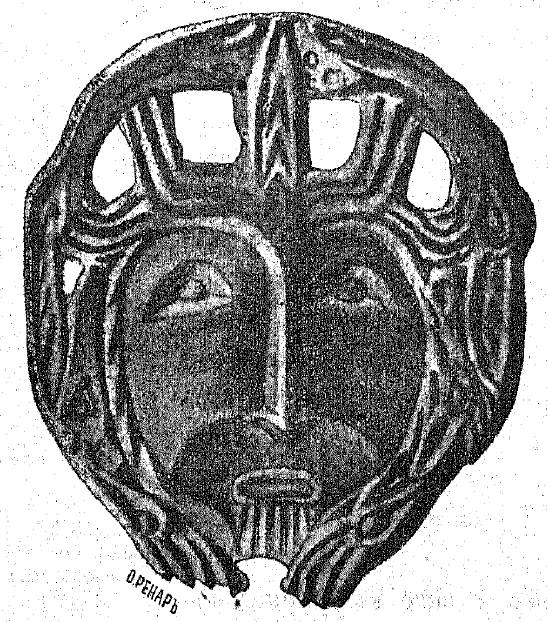
\includegraphics[width=0.80\linewidth]{chast-zmiy/ktotakiezmei/ural-bogi-18.jpg}
\end{center}

Отдельный выступ, составляющий единое целое со шлемом, защищает нос, чем-то закрыт и подбородок. Кожа над верхней губой пилота гладко выбрита. Может это и не пилот, не знаю, с чего я так решил, но в любом случае голова примечательная!

А вот точно пилоты в летательных аппаратах. Модели уже несколько другие:

\begin{center}
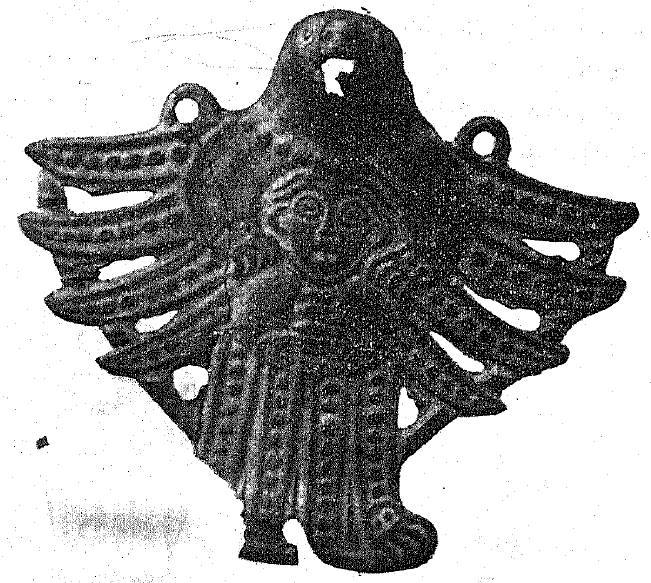
\includegraphics[width=0.85\linewidth]{chast-zmiy/ktotakiezmei/ural-bogi-08.jpg}
\end{center}

\begin{center}
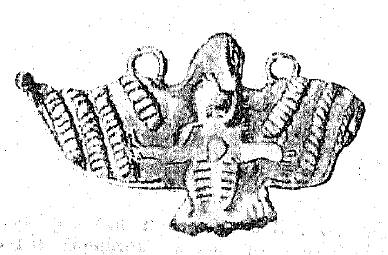
\includegraphics[width=0.85\linewidth]{chast-zmiy/ktotakiezmei/ural-bogi-09.jpg}
\end{center}

У нижней заметно, что правое (на картинке) крыло находится в фазе выдвижения, и тоже состоит из входящих одна в другую пластин. Видно, как пилот держится руками за скобы или рычаги. На аппарате картинки сверху, четко обозначена рама, по которой раскладываются пластины крыльев.

Теперь поглядим на летательные аппараты, давшие повод говорить о множестве голов у змеев.

\begin{center}
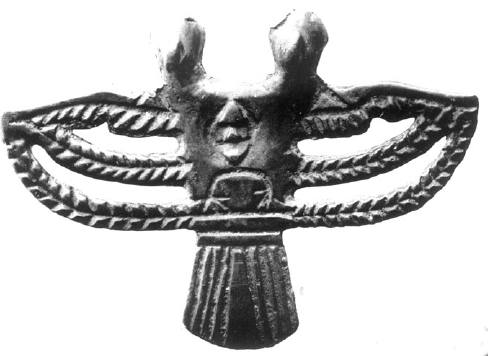
\includegraphics[width=0.70\linewidth]{chast-zmiy/ktotakiezmei/ural-bogi-21.jpg}

\textit{Змей о двух головах.}
\end{center}

\begin{center}
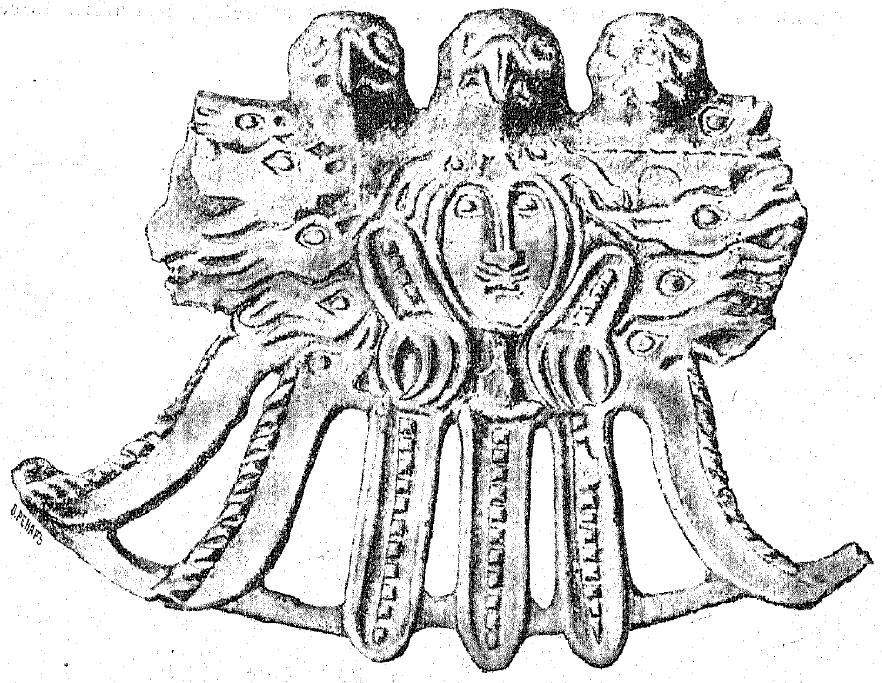
\includegraphics[width=0.70\linewidth]{chast-zmiy/ktotakiezmei/ural-bogi-11.jpg}

\textit{Змей о трех головах.}
\end{center}

Три головы – три турбины, или топливных бака, возможно параллельно им внизу расположены сопла. Обратите внимание, что в середине каждого аппарата – пилоты.

Некоторые бескрылые варианты целиком зависят от двигателей. У фигуры ниже каждая «рука» – сопло, из которого вырывается пламя. Классический реактивный ранец с ракетными двигателями. Дополнительные сопла – снизу, их можно принять за ноги. Без них, фигура имеет очертания современного реактивного ранца.
\vspace*{\fill}
\begin{center}
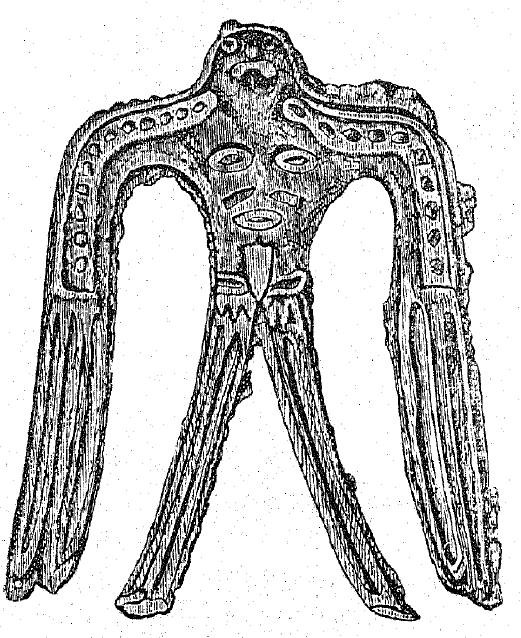
\includegraphics[width=\linewidth]{chast-zmiy/ktotakiezmei/ural-bogi-01.jpg}
\end{center}
\vspace*{\fill}
\newpage

В ходу были и прямоугольные очертания. Сначала покажу рисунок с сосуда, найденного далеко от Урала, в Аризоне:
\vspace*{\fill}
\begin{center}
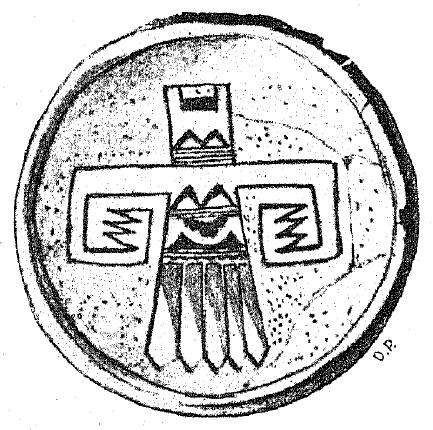
\includegraphics[width=0.65\linewidth]{chast-zmiy/ktotakiezmei/ural-bogi-19.jpg}
\end{center}

И медная бляха из-под Тобольска!

\begin{center}
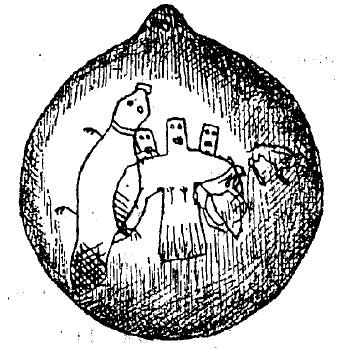
\includegraphics[width=0.65\linewidth]{chast-zmiy/ktotakiezmei/ural-bogi-07.jpg}
\end{center}
\vspace*{\fill}
\newpage

Далее – замечательное двустороннее изображение из меди. Найдено, опять же, в Приуралье.

\begin{center}
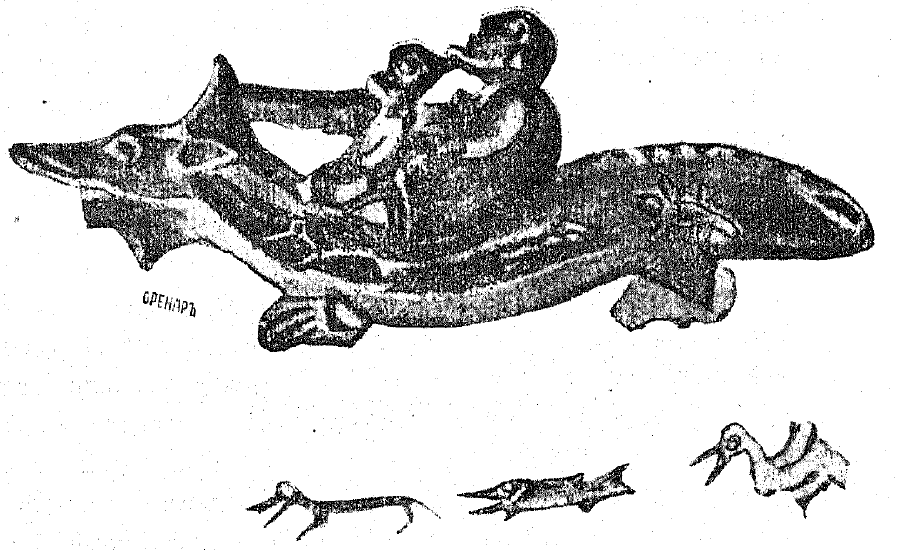
\includegraphics[width=\linewidth]{chast-zmiy/ktotakiezmei/ural-bogi-12.png}
\end{center}

Верхняя часть – лицевая сторона, нижняя – три фигурки с обратной, причем во второй точно показан ихтиозавр!

Ну а сверху – два чудика, один меньший, другой больший, едут верхом на ящере. Головы у чудиков нечеловеческие, либо это шлемы.

Мне сложно представить, что умельцы древности, кем бы они ни были, на всех континентах, сидели и выдумывали фантастических существ, дабы одинаково изображать их в фигурках из бронзы, меди, на глине. Невозможно представить, чтобы они дружно договорились о технологических особенностях летательных аппаратов (рамы с пластинчатыми крыльями, «баллоны»). А может они по косточкам собирали скелеты ихтиозавров и как бы между прочим, легко, воссоздавали их внешний вид на задней стороне медной бляхи?

Нет. Мастера прошлого изображали, отливали из металла то, что видели. Делали это как могли, исходя из своих знаний и художественных традиций. Например, лики на иконах – не реалистичны. Лицо на иконе не передает лицо точно, но изображает его в принятой на то время традиции либо отражает умение художника. Но можно принять за истину, что изображенное в любом случае узнаваемо для современников изображения, а значит, в достаточной мере соответствует подлиннику.

Спросите – а где же наши отечественные фигурки, неужто таких не было? Может и были. Археология нынче такая наука, что на свет вытаскиваются лишь предметы, призванные подкрепить гипотезу автора. Ежели предметы ей противоречат или не нужны, они тысячами лежат в фондах разных институтов, музеев, а то и просто на полках в квартирах. Поэтому черт знает, что нашли, а чего не нашли. Я могу показать только картинки приуральских фигурок, что и делаю.

На летательные аппараты мы поглядели, теперь давайте я вам взлетную площадку покажу.

\begin{center}
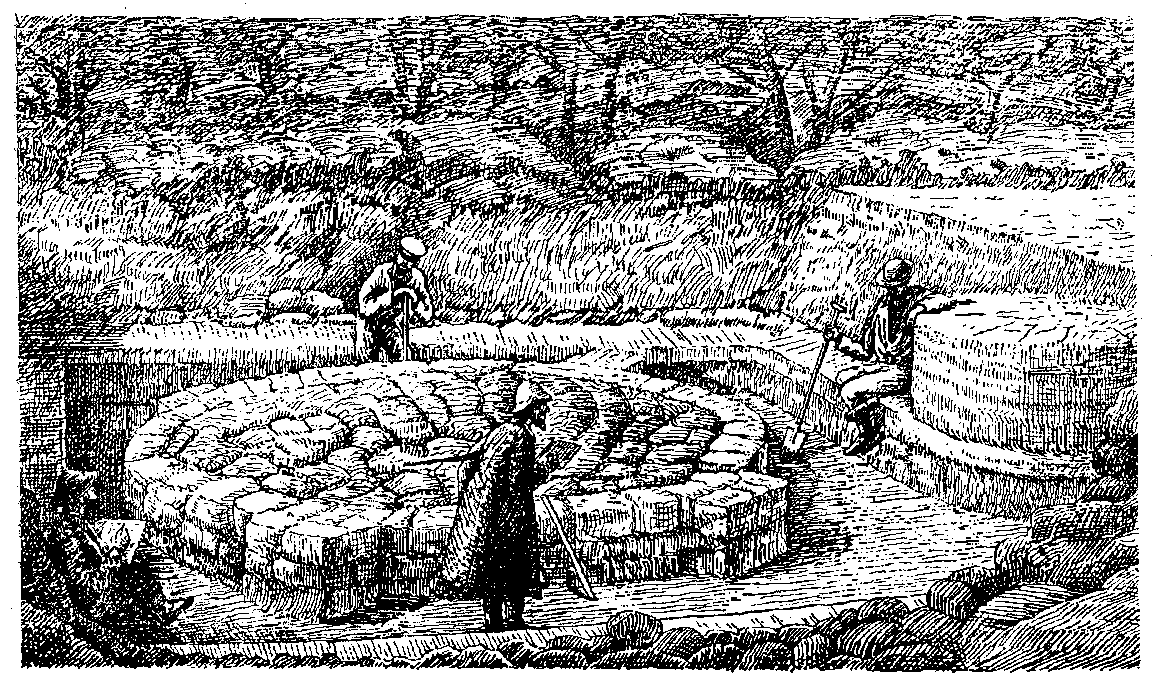
\includegraphics[width=\linewidth]{chast-zmiy/ktotakiezmei/hvoyka-kapishe-01.png}

\textit{Раскопки 1908 г. Рисунок В. Хвойки.}
\end{center}

Да, это знаменитое «капище», отрытое Хвойкой в 1908 году на Старокиевской горе, реконструкцию коего можно сейчас видеть около Исторического музея. Хвойка описывает находку так\cite{hvoyka02}:

\begin{quotation}
Среди остатков различных сооружений, по-видимому, самыми древними являются остатки каменного фундамента какого-то загадочного сооружения. Фундамент этот состоял из различных по величине камней серого песчаника, принимавших иногда причудливые очертания, а иногда имевших сквозные отверстия. Камни эти были сложены на глине, образуя эллиптическую фигуру (4,2 м. в длину и 3,5 м. в ширину), имевшую с четырех сторон по одному четырехугольному выступу (0,7-0,8 м. в длину), которые были обращены по странам света. Вокруг сооружения находился местами хорошо уцелевший пол, вылепленный из толстого слоя беловатой глины с тщательно сглаженной поверхностью. С западной стороны этого фундамента был обнаружен массивный столб, в котором слои сильно обожженной глины чередовались с прослойками золы и угля; вокруг него находилось большое количество костей и черепов животных, главным образом домашних.

Весьма вероятно, что остатки эти принадлежат славянскому языческому капищу, а столб представляет жертвенник, на котором в течение продолжительного времени совершались жертвоприношения, на что указывают многочисленные кости животных и слои глины, чередующиеся с прослойками золы и угля. 
\end{quotation}

Весьма вероятно, это было обычной взлетно-посадоч\-ной площадкой для пилотов, оснащенных небольшими заплечными летательными аппаратами. Если на четырех выступах «капища» поставить какие-нибудь огоньки, получится замечательный ориентир для посадки в темноте. Да и днем хорошо – не скопление же народу дюзами жечь, а на священном месте никто зря топтаться не будет, свободно! Место сие могло одновременно служить и капищем, поскольку сюда приземлялось и отсюда отлетало обожествленное существо.

А тому, пышущему из сопел жаром, просто необходим был этот каменный пятачок – с него удобно взлетать и на него удобно совершать посадку. Каменисто, приподнято, грязи в дождь не будет. Постоянная взлетно-посадочная площадка. Наверное, были и другие, тоже в пригодных местах, на плоских верхушках горных отрогов. Даже без каменного пола. Выйдут волхвы в условленный час, разложат в нужном порядке сигнальные огни – и обожествленный «змей» видит, куда приземляться и где его ждут с дарами-жертвами.

Продолжим про змеев вообще, дабы окончательно разрушить о них представление как о рептилиях, навязываемое учеными, журналистами, писателями, художниками.

Вот Змей Горыныч. Воображение сразу рисует трехголового дракона. Правильно, потому что привыкли, этот образ вдолблен в сознание тысячами иллюстраций и фильмов. А ведь Горыныч, или Горынчич – это от «гора», а не «гореть». Змей из горы. Горный змей. Житель Вятки – он вятич. А обитатель горы – горыныч.

В давнем стихе «Егорий, царевна и змей» бог гневается на три царства – Содом, Гомор и «царство Рахлинское». И вот:

\settowidth{\versewidth}{Напущал Господь Бог на них змея лютого.} 
\begin{verse}[\versewidth]
А на этое третье царство, на Рахлинское,\\
Напущал Господь Бог на них змея лютого.\\
Давали они со города скотиною\\
Ко лютому змею на съедение\\
И ко пещерскому на прожрение.\\
Во граде скота у них мало осталося:\\
Давали они со града по головы,\\
По головы человеческой\\
Ко лютому змею на съедение,\\
Ко пещерскому на прожрение.
\end{verse}

Обратите внимание – змей пещерский. 

Нигде драконоподобие «змеев» не указано, кроме фантазий позднейших авторов. Напротив. Богатыри вскакивают змеям на «белы груди» и грозят зарезать. Змеи разговаривают на русском языке. Во всяком случае, не рычат. Их понимают. Змеи сожительствуют с человеческими женщинами.

В былинах о Вольге (Волхе), змей является отцом этого богатыря-оборотня. В народном стихе «Три года Добрынюшка стольничал» Змей Горыныч (Горынчич) выступает любовником колдуньи Марины Игнатьевны.

Змей, бес, черт, Перун. Не все «змеи» и «бесы» – Перун, но те, кто проявляет себя полетами, громом, молниями, огневой канонадой – определенно. 

Белемниты. Тяжелые, полые, конические штуки с толстыми стенками. Окаменевшие внутренние раковины древних головоногих моллюсков, современников последних динозавров. Похожи на пули или наконечники копий. Какая связь? В народе их называли «перунами» и «чертовыми пальцами», «перуновыми стрелами». Если не знать, что это бывший моллюск, белемнит можно принять за пули и снаряды.

В Древнем Египте их называли «громовыми стрелами» – как это близко к громовержцу Перуну, да и громовержцу Зевсу, тоже метавшему некие стрелы. Еще одна связь с низкорослыми (подобно кумиру Перуна) существами – в странах Скандинавии белемниты слыли «свечами гномов» (vatteljus). В Польше белемниты носят название перуновых камней – kamie piorunowe.

\begin{center}
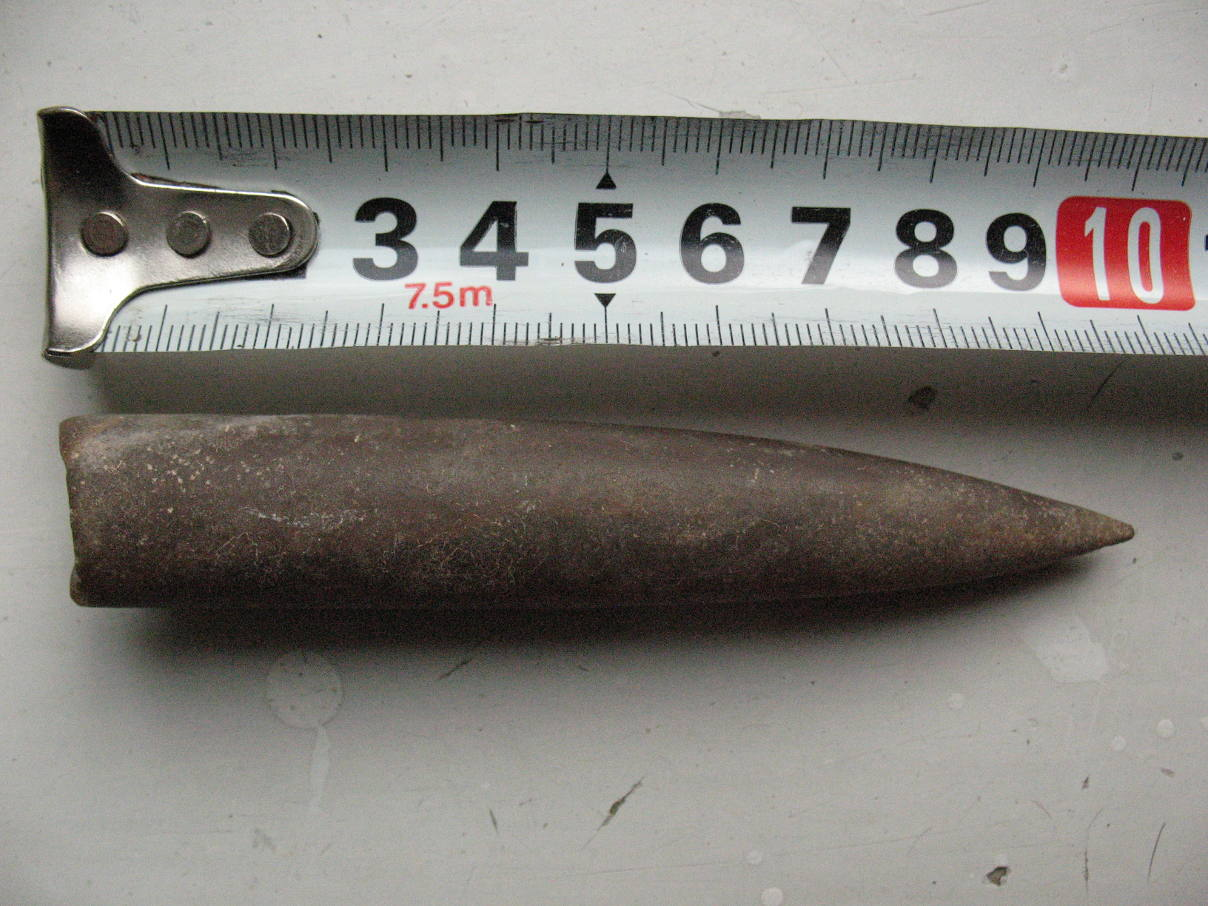
\includegraphics[width=\linewidth]{chast-zmiy/ktotakiezmei/s-IMG_4455.JPG}

\textit{Белемнит с берега Каневского водохранилища близ Трахтемирова (Терех-Темирова). Спасибо Насте!}
\end{center}

Глядя на этот снимок, на ум приходят боеприпасы, пули. И слова «гром», «молния», связанные с Перуном невольно сопоставляются с огнестрельным оружием. Если Перун поражал цель какой-нибудь керамической пулей, отличить её в те годы от белемнита не было возможным. Вот и называли пули и белемниты одинаково – перуновыми стрелами.

Впрочем, есть и такое объяснение – от попадания молнии в песок иногда образуется пальцеобразный предмет, \textit{фульгурит}. Обычно они шершавые и похожи на обломки коралла, но с очень большой натяжкой их можно уподобить белемнитам, и дескать, в народном представлении природа их была едина, от грома!

%Кроме былин и сказок, существует еще вид народного творчества – былички. Прозаические истории недавних времен о необычном. Среди них весьма много рассказов об огненных змеях. Змеев там именуют еще чертями. Часто «змей» не снабжается приставкой «огненный», но просто – змей. Другие названия: летающий змей, летун. 

В народной среде ходило весьма много быличек об огненных змеях. Таких змеев именовали еще чертями. Часто «змей» не снабжается приставкой «огненный», но просто – змей. Другие названия: летающий змей, летун. 

От былинной старины прозаические былички отделены веками. Если былинные змеи – это пожиратели и похитители людей, извечные противники богатырей, то огненные змеи быличек, сохраняя технологичность, меняют свое поведение. Технология же, кажется, становится не такой громоздкой, менее боевой. Бывает, упомянуты даже съемные «крылья».

Змеи деятельно летали над селами и выполняли некие задачи.

Выглядели огненные змеи по-разному. То коромыслом, то как «сноп соломы». Иногда сыпали вокруг искры. Похожие на людей, со съемными крыльями. Приземлившись, змеи обретали человеческий облик. С женщинами, помимо связи половой, вступали в странную – сосали у них кровь из левой груди, за что одаривали деньгами. 

От змеев, по некоторым преданиям, беременели. Такая беременность могла проходить несколько лет. Иногда рождался карлик, уже способный к осмысленной речи, а роженица вскоре умирала. Другие подобные дети просто исчезали невесть куда. А прежде, в сказках и былинах, эти полукровки вырастали героями, обладающими чудесными способностями.

Ходила молва, что некоторым мужчинам змеи носят деньги. Причем змеи, как заправские черти – еще одно подтверждение равенства понятий – заставляли кровью подписывать – нет, не грамоту о продаже души, а договор о получении денег.

Для этого змей надрезал человеку палец. Очень похоже на взятие анализа крови. С той разницей, что у нас в поликлинике за это денег не дают. Змеи меняли деньги на кровавые расписки годами – у человека палец толком не заживал. Будто кровь изучалась на определенном промежутке времени.
 
Что до женщин, жертв внеполового и обычного обольщения огненных змеев, то это были не токмо одинокие вдовы, но и вполне семейные женщины. Они становились бледными, желтыми, худыми, едва передвигали ноги, всё сидели и ждали дорогого гостя. В народе этих змиевых невест кликали солнцевыми девами. Иван Петрович Сахаров «Сказаниях русского народа»\cite{saharov} пишет следующее:

\begin{quotation}
Чародейская песня солнцевых дев, по сказанию чародеев, поется при брачной жизни огненного змея с девушкою. Смешение русских слов со звуками совершенно неизвестными заставляет думать, что она переделана русскими на свой лад\footnote{Мне больше напоминает текст с построчным переводом, а точнее, частичным переводом, где некоторые слова оставлены как были – по неясности или отложенные на потом.}.

«Во всем доме – гилло магал – сидела солнева дева. Не терем златой – шингафа – искала дева; не богатырь могуч из Ноугорода подлетал; подлетал огненный змей. – Лиф лиф зауцапа калапуда. – А броня не медяна, не злата: а ширинки на нем не жемчужены; а шлем на нем не из красного уклада; а калена стрела не из дедовского ларца – Пицапо фукадилимо короиталима канафо. – Полкан, Полкан! разбей ты огненного змея; ты соблюди девичью красу солнечной девы – Вихадима гилло могал дираф. – Из-за Хвалынского моря летел огненный змей по синему небу, во дальнюю деревушку, во терем к деве. Могуч богатырь – Шиялла шибулда кочилла барайчихо дойцофо кирайха дина. – Во малиновом саду камка волжская, а на камке дева мертвая, со живой водой, со лютой свекровью, со злым свекром. Убит огненный змей, рассыпаны перья по Хвалынскому морю, по сырому бору Муромскому, по медяной росе, по утренней заре. – Яниха шойдега бираха вилдо. – А наехал злой татарин и узял во полон солнцеву деву, во золоту орду, к любому Мамаю, ко нехристу бусурманскому, ко проклятому бархадею. – Уахама широфо».
\end{quotation}

Во втором номере «Этнографического обозрения» за 1892 год приведена быличка про змея, который, прибыв к жертве, снимает крылья и втыкает их в крышу – стриху:

\begin{quotation}
Змий – це нечиста сила. Як жинка дуже затоскуе по чоловикови, або шо, от вин до неи и пидкынется, гляды, дукачем, або чим другым. Абы вона тилько ёго у рукы узяла, а то вже вин и почне литаты. Вин у неи з грудей кров ссе... Прылетить, крыла познима, у стриху постромля, та й до неи. Одважиты ёго можна так: як ждешь ёго, сядь на порози, тай розчисуй волосся, наче воши вычисуешь, та для выду покажи, наче б то ты ти воши йисы. Так вин тилько добре шпуртоне тебе, тай подасться геть. Не любе вин того.

(Новомосковский уезд, Екатеринославской губернии). Сообщ. И. Манжура
\end{quotation}

Давайте почитаем и другие, за 19 век, фольклорные записи о змеях. Много их помещено в дореволюционном сборнике «Из уст народа» Гринченко\cite{grinchenko01}.

Кстати, в те годы среди ученой среды, этнографов, принято было считать огненных змеев метеорами. Вопреки описанию свидетелей, произвольным траекториям змеев и так далее. Метеоры!

Объяснили, и спокойно стало на душе. Как с НЛО. Кто хотя бы раз видел НЛО, не станет, подобно сомневающимся, «пояснять» это метеором, северным сиянием, ракетой, особым образом подсвеченными тучами. Но такой человек обычно находит другое толкование, простейшее – инопланетяне. Ни доказать, ни опровергнуть, вопрос веры. 

Одни верят в богов, другие в инопланетян, третьи в природные явления. Но чувство внутреннего уюта заслоняет ощущения внешние. Так мы закрываем ладонями уши, услыхав громкий, раздражающий звук. Звук не исчезает из действительности, но пропадает для нас и более не мешает.

Не знаю, кого или что называли селяне огненными змеями - пилотируемые аппараты «былинного типа», дроны, каких-то существ в костюмах для полетов, или существ или аппараты из неведомых видов материи, либо не материи вовсе.

\begin{quotation}
Я уже не докажу, куды той змий летив и кому вин нис гроши, – кажуть люде, що вин носыть тому шевцю, що на краю села\footnote{Еще бы – на окраину летать удобнее, не столь заметно, как посреди селения.} – а що свойимы очыма бачыла, як вин летив. Я йшла додому, колы летыть – довгый, довгый, икраз як коромысел; стала я к плетню и нагнулась, бо вин так нызенько летив, та усе и хыляеться, та блестыть же так! Чуть-чуть не зачепыв мене и пролетив удовж села.

М. С. Чудновская от крестьянки г. Березного Черниговского уезда, 1898
\end{quotation}

\begin{center}
***\end{center}

\begin{quotation}
Багато нас, хлопцив, йихало на ночлиг и бачылы, шо змий, увесь красный та блыскучый, то подыметься вгору, то знов опустывся и так до трох раз, а у трейте пиднявся и полетив. Мы бачылы, як вин пролетив скризь церкву и повернувся до П-ча. Кажуть, що сьому чоловику змий носыть гроши.

М. С. Чудновская в с. Выблях, Черниговского уезда, от Демьяна Конопки в 1890 году.
\end{quotation}

\begin{center}
***\end{center}

\begin{quotation}
Одын чоловик ишов селом и бачыв, як над його головою пролетив змий – икраз як куль соломы, а з того куля так и сыплються искры, и вин так увесь и сяе. Чоловик дуже злякався, та все такы хотив подывыться, кому се змий несе гроши. Аж вин так и полетив на куток, и як долетив до Б. хаты, то де й дився, тилькы дым пиднявся вгору.

М. С. Чудновская, в с. Выблях, от Захария Леуса, в 1898.
\end{quotation}

\begin{center}
***\end{center}

\begin{quotation}
Мий батько був раз обходчыком. Иде вин с другым и бачыть, що на стреси у однийи бабы щось блыщыть, наче жару насыпано. Пидийшлы воны блыжей, щоб розглядить, що воно таке, аж из хаты выйшла хазайка, щось промовыла, и тее блыскучее загуло так страшенно и провалылося\footnote{Некое взаимодействие хозяйки хаты и змея!}. Кажуть, що се змий носыть гроши сий баби, а баба та – видьма: вона и змия прыймае до себе, и з нечыстою сылою знаеться.

М. С. Чудновская в с. Выблях, от Петра Муцкого, 1898.
\end{quotation}

\begin{center}
***\end{center}

\begin{quotation}
У одний хати зависылась молодыця, и став туды що ночи литаты змий. Прилетыть було, покладе коло хаты крыла\footnote{Опять эти съемные крылья.}, а сам зробыться чоловиком и йде у хату.

Постериг раз челяднык, як змий скынув крыла, и зробыв так, як раелы люде: перехрестыв йих. Выйшов чоловик той з хаты, да не может узять крыл, а давай вин кланяться та просыть наймыта подать йому крыла.

 – Насып, – каже наймыт, мени повну шапку грошей, тоди подам.

Став змий сыпать у шапку гроши, а шапка да була з диркою. Насыпав уже стилько, що аж пид самый бовдур.

 – Ну, – каже тоди наймыт, – на твои крыла, та бильш до нас не литай, бо останешся без крыл.

М. С. Чудновская, в с. Выблях, от Владимира Ковпыты, в 1898 г.
\end{quotation}

\begin{center}
***\end{center}

\begin{quotation}
Ученые не вирять, що сатана может зробыться чым завгодно и йиздыть, чы там летать до того, кого все уподобае, адже ж сьому правда.

Мени самий хоть и не траплялось бачыть, а багато людей росказують, як у опивнич велычезный, як коромысел, та блыскучый, мов золотый, змий летав до Б., того чоловика, що живе на конци села\footnote{И снова – змей летает в окраинное жилище.}. Не скажу все, як воны потоварышылы, и змий помився сьому чоловику наносыть мирку грошей. Б. забажалось грошей ще бильш вид миркы; выкопав вин у хливи глыбоку яму и всунув туды бездонну зелизну мирку. Став змий що ночы летать до того чоловика и насыпать ту мирку грошыма; тилькы як вин не стараеться насыпать повну, – нияк та й годи!

А дали змий якось то уже прыдывывся, що мужык його одурыв и що грошей там уже багато, не миркою пахне.

Росердывся тоди змий, звелив мужыку уризать палца и кровью роспысаться, що гроши вин получыв; а тоди спалыв у того мужыка раз, спалыв удруге, и давай його що гору палыть\footnote{То есть, змей устраивал пожары.}.

Люде и прымитылы, що як уже усе кончыться, позалывають, бере тоди сей чоловик заступ, выкопае гроши и клунками тоди уже з сынами й носыть и друге мисто. Опротывело чоловикови горить та таскаться з тымы грошыма, и давай вин хвалыться людем, що «так и так, каже, наносыв мени змий грошей, а теперь палыть, – що його в свити диять?».

Ну, звисно, у кажному сели е таки люди, шо вид усього знають, и пораялы воны йому кажень рик робыть яку небудь новую прыстройку, чы там хлив якый, чы повитку, чы покривлю перекрыть, абы то що небудь нове.

И с тых пор перестав той чоловик горить. Вин и теперь жив, палець у його и доси не зрисся и робыть вин так, як йому раялы люде; тилькы, звисно, уже збиднив, бо килькы раз горив, подилывся з сынами, к тому ж и дорогу до шынку добре знае, та такы, правду кажучи, де то все дыявольськымы грошыма й забагатиеш?

М. С. Чудновская от Хведоры в с. Выблях, Черниговский уезд.
\end{quotation}

Немало подобных народных рассказов приводит В. П. Милорадович в «Заметках о малорусской демонологии» (Киевская старина, 1899, тома 8, 9):

\begin{quotation}
Я ще дивкою бачыла змия. Идем з подругами з улыци додому, то вин летыть з-за Сулы, такый, мов жменя конопель. (Литвяки)
\end{quotation}

\begin{center}
***\end{center}

\begin{quotation}
Летив вин, як вязка соломы, я упала ныць. (Пески)
\end{quotation}

\begin{center}
***\end{center}

\begin{quotation}
Я на вику чотыры раза бачыв змия: первый раз стояло нас на юлыци шисть парубкив. Колы, де й вин узявсь, летив клубком и обсыпав нас искрамы. Полетив на провалля. 

Другый раз ишов я сам на юлыци, спиваю. Вин мов з Чумакова двора на Марьин сад полетив. Летив нызько, такый, як мих ковальский\footnote{Форма капли, положенной на бок.}. 

Третий раз нас двое и дви дивчат гулялы. Летив вин нызько з Якымовои левады. Род дныща, роспарусывсь\footnote{Парусами называли также крылья ветряных мельниц и плавники.}, и искры мали. 

Четвертый раз я волы пас. Летив вин тоди найвыще з Снитина на Стинку. Мов угору на вныз, як горобець. (Снетин)
\end{quotation}

\begin{center}
***\end{center}

\begin{quotation}
Бачыв змия; як сорока, и стать, як сорока. Нос довгый. Искрыть дуже наперед и назад. Зайшов за хмару. (Лазирки)
\end{quotation}

\begin{center}
***\end{center}

\begin{quotation}
Двичи бачыла змия: голова – клубок, а дали мотовыло. Згынается, як гадына. Нызько летив, искрыв. (Пятигорцы)
\end{quotation}

\begin{center}
***\end{center}

\begin{quotation}
Летило таке, як заступ. Упало, мов дижа. (Войниха)
\end{quotation}

\begin{center}
***\end{center}

\begin{quotation}
Сыдила я на поли, и поз мене загуло, неначе човен, так як сонце зийшло. Вин не вглядив. (Пески)
\end{quotation}

\begin{center}
***\end{center}

\begin{quotation}
Дивкою двичи бачила змия. Голова велыка, як дижа. Довге, страшне, сидало на выгони. (Литвяки)
\end{quotation}

\begin{center}
***\end{center}

\begin{quotation}
Змий летив такый, як коромысло, и вгору и вныз огонь розсыпа, сажня чотыри вышыны, и полетив вдовш села. Пид животом мав червоне, крыламы маше, огонь сыпле. (Хитцы)
\end{quotation}

\begin{center}
***\end{center}

\begin{quotation}
Летыть, так и ося оселю. Довгый, так я чоловик, роспарусыться, так з ёго огонь и креше. (Литвяки)
\end{quotation}

\begin{center}
***\end{center}

\begin{quotation}
Посидалы мы на юлыци, колы змий летыть та аж прызырается. Бильш аршына удовш. Парусы таки, мов у коня хвист. (Снетин)
\end{quotation}

\begin{center}
***\end{center}

\begin{quotation}
Йихав я у Снитин на Мызиновку. Змий сив на ярмо. Голова и все у ёго аж осияло, булы миста по ёму и чорни. Быкы жахнулысь, бигты, я вдержав их, перехрестывсь, а вин знявся и полетив. (Литвяки)
\end{quotation}

\begin{center}
***\end{center}

\begin{quotation}
Заспивав вечирашний пивень, а дивци здалось, що вже досвичаный. Схопылась вона, убралась: «Пиду вже я, мамо». Маты спыня: «Не иды, по ще рано». «Проведить мене хоть тришечкы: я пиду у строк». Маты ии вывела з улечки: «Иды, дочко, не бийся, тилькы хрестысь».

Вона соби иде, иде, увийшла так як верст дви, колы це перед нею як и посыплются зори, так ии стане аж у вичи жовто, не выдко куды йты. Вона злякалась; пидийшла так из гоны, колы лежыть плитка серебряна, побильше ложкы. Стане дивка переходыть колию, то й плитка перескочыть и впаде. То дивка та перейде впять у ту колию, и плитка впять перескоче и ляпне.

А дивка вже и излякалась, сама соби каже: «Господы мылостывый! Мени маты казала – хрестысь, а я й забулась». Стала хрестыться. Так вин тоди огнем як заискрывсь. Як заступ зробывсь из тии плиткы, рванув бурею, каже: «Догадлыва!». А вона впала и лежала досвита; прыйшла утром, уже робочи снидалы. Лежала тыждень, схвачувалась. Вылывалы переполох: вылывалась так рыба из парусами, як вин пидкыдавсь та искрыв перед нею.

с. Литвяки, казачка Д. Бугаева.
\end{quotation}
 
Сравнение змея с коромыслом встречается в быличках неоднократно. Для городского жителя коромысло представляет довольно отрешенное понятие, такое же как скажем «гумно». Ну коромысло так коромысло, все знают, как оно выглядит. Дуга такая, на ней ведра носят.

А если это подробно вообразить?
\begin{center}
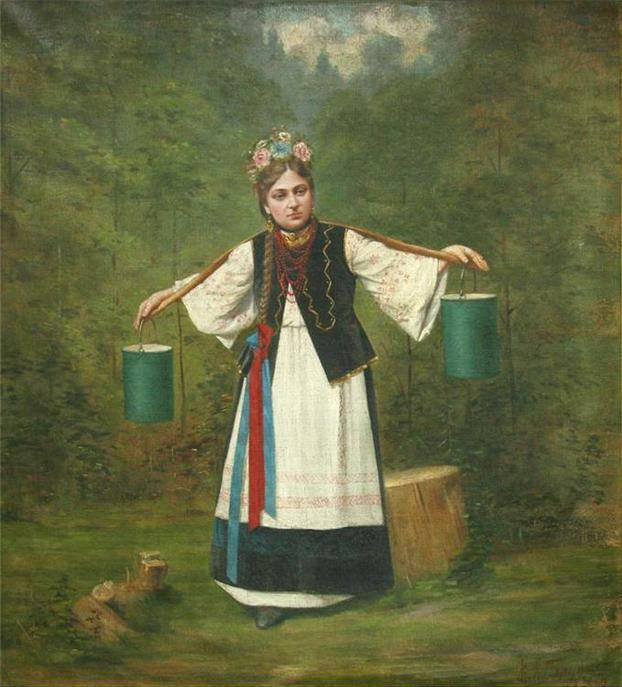
\includegraphics[width=0.50\linewidth]{chast-zmiy/ktotakiezmei/koromyslo_malyavin.jpg}

\textit{Женщина с коромыслом. Ф. Малявин.}
\end{center}
\newpage

\begin{center}
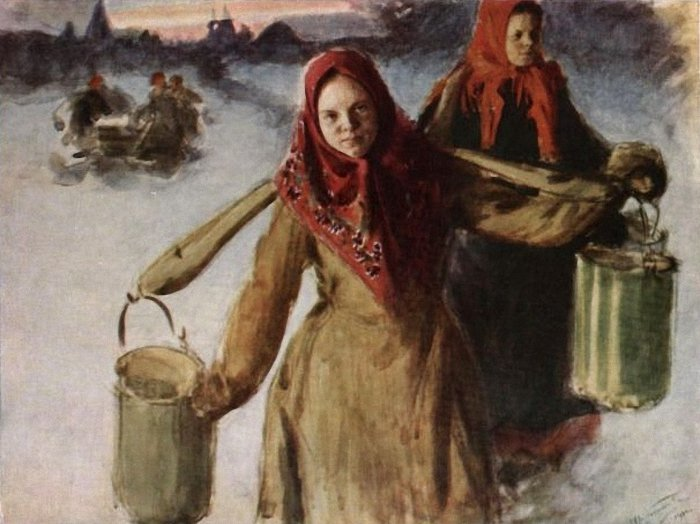
\includegraphics[width=\linewidth]{chast-zmiy/ktotakiezmei/koromyslo_kulikov.jpg}

\textit{За водой. 1904, Куликов И.}
\end{center}

\begin{center}
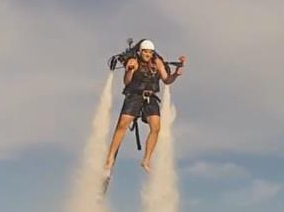
\includegraphics[width=\linewidth]{chast-zmiy/ktotakiezmei/jetlev_jetpack.jpg}

\textit{Ракетный ранец Jetlev, 2012, фото Seg9585.}
\end{center}

\newpage

Сравним образ девушки с коромыслом да современные и не очень, ракетные ранцы. 

\begin{center}
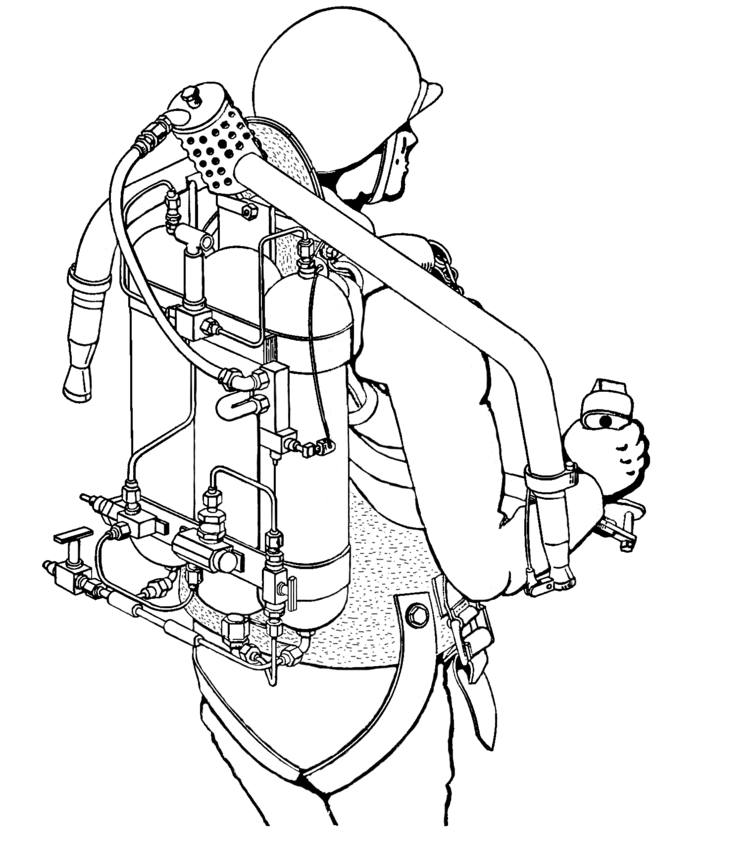
\includegraphics[width=0.86\linewidth]{chast-zmiy/ktotakiezmei/rocketpack_general_view.jpg}

\textit{Американский реактивный ранец 1960-х годов Bell Rocket Belt Уэнделла Мура, вид сзади.}
\end{center}

К сожалению, по причине пресловутых авторских прав я не могу использовать здесь фотографии, которые подошли бы для иллюстраций лучше. Что нашел в открытом доступе, то и пускаю в ход. На других снимках, которые не попали в книгу, есть такие, где контуры пилота с ранцем совершенно повторяют женщину с коромыслом! Вёдра это турбореактивные двигатели, коромысло – их крепление, за спиной – баллоны. Я не утверждаю, что «змеи» использовали именно такую технологию, но внешне сходную.

\newpage

В былинах часто говорится о неких «хоботах» у змеев. На следующей иллюстрации – не это ли обозначали сказители метким словом?

\begin{center}
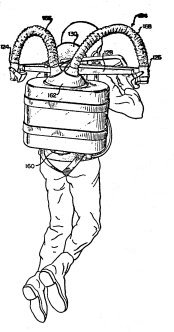
\includegraphics[width=0.40\linewidth]{chast-zmiy/ktotakiezmei/rocbelt-3.jpg}

\textit{Американский реактивный ранец 1960-х годов, вид сзади.}
\end{center}

\begin{center}
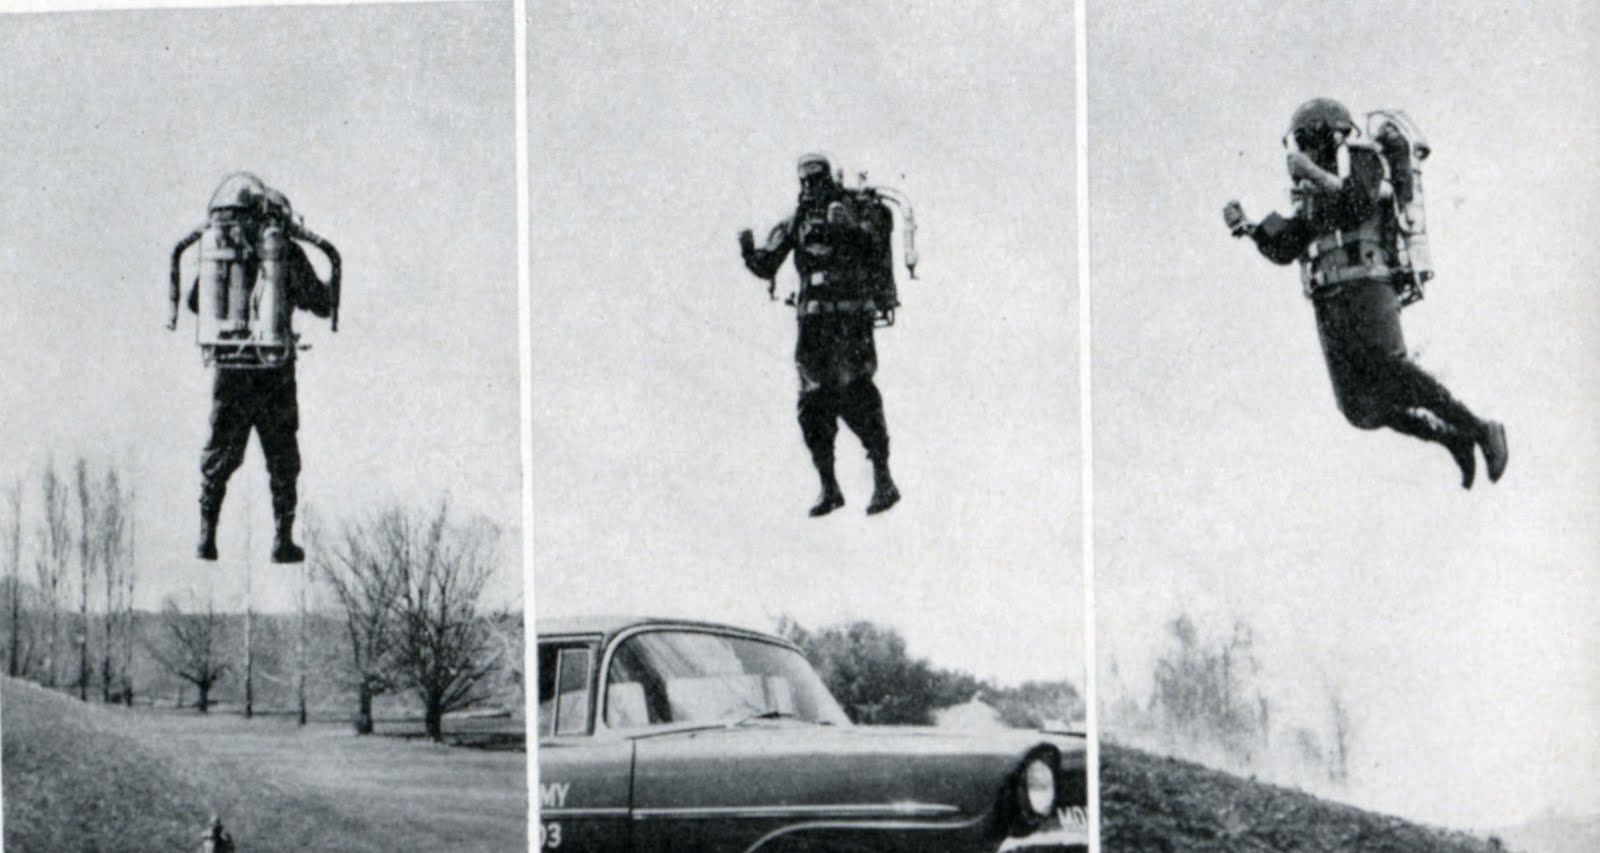
\includegraphics[width=\linewidth]{chast-zmiy/ktotakiezmei/1962Eaglebookofhowitworks03.jpg}

\textit{Тестирование ранца Bell Rocket Belt, 60-е.}
\end{center}

Существуют ранцы, которые выглядят и коромыслом именно с ведрами, желающие могут легко убедиться в этом посредством Сети. С крыльями и без, на основе различных двигателей, современные «летучие ранцы» всё еще хреново летают, стоят дорого и относятся более к экспериментальным причудам, нежели к технологии, пригодной для повседневного использования хотя бы спасательными службами.

Александр Федорович Андреев придумал подобный ранец, на бумаге, в 1919 году – сохранились документы. Гитлеровцы вроде хотели поставить свои ранцы на конвейер – не вышло, потом эстафету перехватили американцы, но толку по сей день мало – небольшое время полета для быстрых моделей, опасность перегрева для пилота, либо, напротив, медлительность, как в случае «водного» ранца Jetlev-Flyer. От Jetlev в воду тянется тоже хобот – шланг, присоединенный к плывущему за аппаратом скутеру, подающему по шлангу воду под давлением. Jetlev-Flyer это гибридная технология для развлечения, не «чистый» реактивный ранец.

Итак, аттракцион и экспериментальные модели.

Но задолго до того, как человечество узнало о реактивных ранцах, те, кого в народе называли змеями, кажется использовали подобные аппараты на всю катушку!

Не зря, думаю, забавные воздушные змеи, запускаемые детьми и взрослыми на бечевках с земли, именуются именно змеями. Не бумажными птицами, а именно змеями.

Узкие полосы, из которых составлялись крылья летательных аппаратов на «чудских» фигурках навели меня на мысль о происхождении слова «Перун» – оно производно от «перо». 

Без досужего языковедения, когда на всякий лад доискиваются до смысла корня «пр» или «пер», я предлагаю толковать буквально. Ведь «перо» не связано непременно с птицей. Зеленое перо торчит из луковицы. Пером называли плавники у рыбы. Перо еще также – нож. Стало быть, «пером» обозначали нечто удлиненное и плоское. Под это описание подходят и выдвижные пластины из крыльев летательных аппаратов змеев.

Наблюдаемые людьми перемещения «змеев» совершались с целями – беспрепятственно посетить нужного человека, выполнить по отношению к нему некое действие, иногда отдать взамен подарки либо деньги, и улететь.

Порой, огненный змей проникал к жертве через предмет, ею подобранный – например, это мог быть перстень или ожерелье. Принесенный домой, такой предмет превращался затем в «паныча» (то есть  выглядел господином), либо служил маяком, по которому на место является змей. После, уже традиционный огненный змей начинал еженощно посещать дом или сарай, смотря где женщина спит, обращался в «пана» и сосал из груди кровь, а жертва чахла. 

Превращение предмета в паныча происходило неявно. Положит, скажем, девушка найденное колечко в сундук, потом открывает – а там уже паныч! Возможно, предмет просто нужен для пеленга.

В быличках России вместо «паныча» змей обращается «добрым молодцем». Иногда это безымянный змей, иногда сам Змей Горыныч: «прилетает к реке Змей Горыныч; ударился о сыру землю и сделался таким молодцом, удалым красавцем». Прилет и посадка змея сопровождается воздействием на окружающую среду: «вдруг деревья в лесу зашумели, крыша на избе пошатнулася».

Само превращение змея в паныча заключалось в скидывании крыльев. Совершив без крыльев задуманное, паныч снова оборачивался в змея, надевая крылья. Именно крылья связаны с «огнем», а их использование для отлета описывается словами «здвынувся», «бурею пишов» и тому подобными.

Некоторых змеев вроде бы легко обмануть – в быличках встречаем, что змей не распознает притворство, как больших кукол принимает за живых людей, если ему сказать, будто это гости на свадьбе, и так далее.

Листая и сборники сказок, иногда сталкиваешься с обыденностью в описании «змеев» – примерно то же ощущение испытываешь, читая ирландские предания, где просто, без желания удивить рассказывают о персонажах из волшебного народа. 

В сказке «Змиева дочка»[вып. 1]\cite{grinetnochern} из сборников Гринченко один богач отправляется в другую страну, где мало воды, и просит там у царя воды. Взамен царь обманом выдуривает у богача сына. Потом этот сын отправляется к царю, и оказывается, что «цар той був сам змій и знав багато чарів, а найменша дочка була ще більша чарівниця од батька». В итоге царю-змию рубят голову над колодцем, а сын богача женится на змиевой дочке. 

Рудченко приводит\cite{rudskazki} несколько сказок под заглавием «Змий», обе – распространенная быличка про летучего змея, соблазнителя, и в первой змий прямо отождествляется с чертом. Еще одно именование огненного змея – огненный бес.

Про змеев-любовников знали не только в 19 веке, когда этнографы стали записывать былички, но гораздо раньше. Существует русский литературный памятник «Повесть о Петре и Февронии», написанный Ермолаем Прегрешным (в иночестве Еразмом) в 1540-х годах.

В основе лежит народное предание, церковью и учеными привязанное к историческому лицу, князю Давиду Юрьевичу Муромскому (1203/1205-1228).  Кроме предания есть источник, предшествующий написанному Еразмом житию – 15 века служба святым Петру и Февронии, созданная Пахомием Сербом. В тексте службы упомянута победа над змеем. Подробный разбор вопроса тождественности Давыда и Петра читайте в работе М. Скрипиля «Повесть о Петре и Февронии в ее отношении к русской сказке»\cite[том VII]{trudy-aknauk-otdel-drevsuslit} – там же и полезный свод источников.

Классический вариант повести от Еразма\cite[стр. 454-463]{izbornik01} начинается так:

\begin{quotation}
Се убо в Русиистеи земли град, нарицаемыи Муром. В нем же бе самодержавствуяи благоверныи князь, яко поведаху, именем Павел. Искони же ненавидяи добра роду человеческому, диявол всели неприязненаго летящаго змия к жене князя того на блуд. И являшеся еи яков же бе естеством, приходящим же людем являшеся своими мечты, яко же князь сам седяше з женою своею. Теми же мечты многа времена преидоша, жена же сего не таяше, но поведаше князю мужеви своему вся ключшаяся еи, змии же неприязнивыи осиле над нею.
\end{quotation}

К жене князя Павла летал змей, принимал образ самого князя и занимался с нею блудом. Супруга князя ничего от мужа не утаила, и тот стал думать, как дальше быть. Сообразил. Говорит жене – подластись к змею и спроси, мол, как его убить можно. Княгиня поступает согласно совету. Змей однако доверчив.

\begin{quotation}
Он же неприязнивыи прелестник прельщен добрым прелщением от верныя жены, яко непщева таину к неи изрещи, глаголя: «Смерть моя есть от Петрова плеча, от Агрикова же меча!»
\end{quotation}

Княгиня передала слова змиевы князю. А у того был богомольный брат Петр. Князь поведал ему про змея, и Петр принял это на свой счёт. Стал мыслить, как же ему змия убить. Что за Агриков меч такой?

Петр имел обыкновение в одиночестве ходить по церквям. Повесть говорит, что: 

\begin{quotation}
Бе же вне града церковь в женьстем монастыри Воздвижение честнаго и животворящаго креста. И прииде к ней един помолитися. Яви же ся ему отроча, глаголя: «Княже! Хощешили да покажу ти Агриков мечь?»

Он же хотя желание свое исполнити рече: «Да вижу, где есть!» Рече же отроча: «Иди вслед мене». И показа ему во олтарней стене межи камения скважню, в ней же лежаще мечь. Благоверный же князь Петр взем мечь той и прииде и повода брату своему. И от того дни искаше подобна времени да убьет змия.
\end{quotation}

Явления чудесных отроков (отроками считались дети до 14 лет, возможно, в описании «чудесных отроков» речь идет скорее о росте, чем о возрасте), передающих послания\footnote{Словом «аггел» (ангел), кстати, Греки переводили тоже «посланника», из подлинника Библии.}, в русской религиозной литературе, во многом по сути документальной – не редкость.

Что же, Петр берет из тайника меч и через некоторое время отправляется к брату и снохе. Повидался сначала с братом, князем. Сразу от него идет к снохе – а там снова сидит брат. Понятное дело, то змей в образе князя, но Петр не понял и оставил покои княгини. На обратном пути встретил человека, сказавшего ему, что князь никуда из своей храмины не выходил, княгиню не посещал. Петр вернулся к настоящему князю, удостоверился – брат на месте, попросил его уж точно никуда не двигаться, и – 

\begin{quotation}
И взем мечь, нарицаемый Агриков, и прииде в храмину к сносе своей, и видев змия зраком аки брата си, и твердо уверися, яко несть брат его, но прелестный змий, и удари его мечем. Змий же явися яков же бяше естеством и нача трепетатися и бысть мертв и окропи блаженнаго князя Петра кровию своею. Он же от неприязнивыя тоя крови острупе, и язвы быша, и прииде на нь болезнь тяжка зело. И искаше во своем одержании от мног врачев исцеления, и ни от единого получи.
\end{quotation}

После смертельного ранения змей преображается из князя в свой истинный облик – повесть умалчивает его. Умирая, змей своей кровью окропил Петра. Тот покрывается струпьями, язвами, и тяжело болеет. Описание похоже на лучевую болезнь.

Петр ищет лекарей, наконец ему в веси Ласковой, что в пределах земли Рязанской, отыскали странную девицу Февронию, дочь древолазца (отец с братом ея лазали в лесу на деревья за медом), что говорила загадками, а вокруг нее по дому скакал заяц. Народный рассказ, записанный под Смоленском, именует Февронию «богатыркой».

Феврония вызвалась врачевать князя Петра, если он возьмет ее в жены. Петру жениться на «дщи древолазца» не улыбалось, однако на словах согласился. Феврония снабдила его сосудцем некой кисляжди и приказала идти в баню и намазать там струпья и язвы, ничего не пропустив.

\begin{quotation}
Наутрие же узре все тело здраво и гладко, разве единого струпа, иже бе не помазан по повелению девици. И дивляшеся скорому исцелению. Но не восхоте пояти женою себе отечества ея ради и посла к ней дары. Она же не прият.

Князь же Петр поеха во отчину свою, град Муром, здравствуяи. На нем же бе един струп, еже бе не помазан повелением девичим. И от того струпа начаша мнози струпы расходитися на теле его от перьваго же дни, в онь же поехал во отчину свою. И бысть оструплен многими язвами, яко же бе и первие.
\end{quotation}

Тогда князь Петр вынужден был воротиться к Февронии, согласился на женитьбу и получил то же снадобье, что и в первый раз. Условием Февронии являлась именно женитьба. Полагаю, девица хотела быть княгиней, взамен снабжая князя своим лекарством, которое действовало лишь некоторое время, а не потому, что «един струп» был пропущен. Налицо соглашение – статус княгини в обмен на постоянное лечение.

Новоиспеченные супруги едут на отчизну Петра, в Муром. Вскоре князь Павел умирает, и Петр становится единым в Муроме самодержцем. Повесть продолжается, но в ней более нет о змеях, поэтому я, как Шахерезада, прекращаю дозволенные речи!

В этой огромной главе я хотел приготовить вас к восприятию былин, отличному от привычного – мол, богатыри сражаются с драконами. Нет драконов! В слово «змей» вкладывается ровно тот смысл, как мы прочитали в быличках, преданиях. Предания эти были сходны по всей Руси, отличаясь более по времени, нежели по местности. Былинные змеи – больше «боевые», а змеи быличек – собиратели крови и прелюбодеи, либо просто летуны.

Например, былички, собранные во второй половине 20 века Зиновьевым в Сибири\cite{zinoviev01} ничем, кроме языка, не отличаются от украинских, 19 века быличек про змеев. Приведу и несколько устных рассказов из книжки «Предания и легенды Урала» (1991), составленном В. П. Кругляшевой. Они носят уральский отпечаток, но по сути одинаковые с быличками о змеях из любой другой местности:

\begin{quotation}
[...] Был у меня один хороший знакомый. Раньше он золото добывал, а года три назад умер. Так он видел такого змея. Шел как-то пьяненький из кабака, идет, песни поет. Глядь, а по нему летит змей огненный. Страшный такой, искры летят во все стороны. Небо светлое от огня его сделалось. Все смотрят, крестятся. Упал он где-то в лесу, а через два года нашли в том лесу клад очень богатый. [...]

Зап. в д. Полдневой от И. И. Иванихиной, 1904 г. р.
\end{quotation}

\begin{center}
***\end{center}

\begin{quotation}
Ехал как-то мой отец, тогда еще мальчонка, с дедом по лесу. Вдруг глядят, а за ними шар огненный летит, весь так и пылает, и сзади его хвост горящий мечется. А дед-то умел нечистую силу заговаривать.

Поговорил он каких-то слов непонятных, шар-то и остановился, присел к ним на сани на самый зад, сидит тихонечко. Дед спрашивает: «Куда летишь?». Нечистый и отвечает: «Есть тут вдовушка одна, все тоскует, все плачет, меня зовет. Я и лечу ее утешить». А дед ему: «Чтоб ты не смел, нечистый дух, больше и появляться, не то я тебя поражу». То ли вправду дед власть над ним имел, то ли еще что, но только сполз этот шар с саней да и тут же растаял, словно его и не было, и больше уж в дедовой деревне не появлялся. [...]

Зап. в г. Кушве от П. М. Авдониной, 1903 г. р.
\end{quotation}

Любопытно, что в Новгородщине с огненными змеями отождествлялось слово, близкое к Перуну – пар\'а. В первом томе «Живой старины» за 1896 год  есть заметка «Летучий огненный змей», М. А. Синозерского, где впрочем явление огненных змеев приписывается сочинителем заметки к неким «падающим болидам». Однако приведу выдержку:

\begin{quotation}
15 марта, 1895 года, в 9 часов вечера, над ст. Померанье, Новгородского уезда, пролетел по направлению от юго-востока к северо-западу необыкновенной величины болид, оставивший на пути полета продолговатую светящуюся беловато-фиолетового цвета полосу. Свет происходящий от трения болида об воздух, был настолько силен, что затмил свет лампы и свечей в домах.

Перепуганные жители села выскочили на улицу, но увидели только одну световую полосу на небе. В народе поднялись толки о только-что бывшем явлении. Между прочим одна баба уверяла другую, что видела, как огненный змей с большим хвостом пролетел по воздуху.

Заинтересованный этим объяснением небесного явления, я, прийдя с улицы домой, спросил свою квартирную хозяйку-крестьянку: «что это за змей, который летел сегодня по воздуху?».

Она ответила, что это «пар\'а летит».

 – Что такое «пара»?

 – «Пара?! – Это нечистый дух».

 – Куда же он летел?

 – «А кому-нибудь деньги понес».

   Расспросив ее обстоятельнее, я узнал, что «пара» по народному поверью, летает по ночам в виде огненного змея к тем людям, которые с ним знакомы, и носит им золото, от чего они богатеют. Так что, если какой-либо человек неожиданно разбогател, то народ говорит, что ему «пара» денег наносил.

На вопрос мой, видала ли она «пара», хозяйка отвечала, что видала раз, возвращаясь с гумна, как сзади что-то осияло. «Тут все» (идущие с ней) «сказали, што это »пара« полетел».
\end{quotation}
 
В «пар\'а летит» мне явственно слышится искаженное «Перун летит».
 
Перейдем к более давним временам, о коих повествуют былины и предания. Былины о Киеве, так называемый «киевский цикл», записаны не в Киеве, а в местах от него отдаленных – Север России, Сибирь. Куда девались былины на землях Украины, вопрос отдельный.
